%%% ----------------------------------------------------------------------
\section{Stage 5, the Faces: Flat Charts Known Only by Their Edge Lengths}
\label{section:int_triangle}

\paragraph{What we want.} Stage 5 is the discretization: the mesh and the finite dimensional space. Stage 4 ended with three ingredients that Stage 5 must supply: the metric, the rotation gauge and the transitions between charts. This section supplies the first two on each face. The chart of a face is the reference triangle, or the layout of the face in the plane, and its displacement gauge is the same at every point of the face. We want to show two things. First, everything the finite element method needs from a face, other than the transitions, is a function of the three edge lengths, and we compute it from them. Second, in the chart of a face the rotation gauge vanishes.

\subsection{The metric of a face is its Gram matrix}

Recall from Section~\ref{section:gradients} the affine map from the reference triangle to the face,
\begin{equation*}
F(\xi) = x_1 + B\, \xi, \qquad B = [\,x_2 - x_1 \;\; x_3 - x_1\,] = [\,e_1 \;\; e_2\,],
\end{equation*}
with $B$ a $3 \times 2$ matrix. In the language of Section~\ref{section:r3_displacement}, the reference triangle is the chart of the face and $B$ is its displacement gauge: the map~(\ref{eqn:r3_h})~[\,$h(a) = a_1\,\partial x/\partial\xi_1 + a_2\,\partial x/\partial\xi_2$\,] is $h(a) = B a$, since $\partial F/\partial\xi_1 = e_1$ and $\partial F/\partial\xi_2 = e_2$. So $h = B$, constant on the face. The matrix $B$ contains the full position of the face in space. We ask what part of $B$ is needed to measure lengths on the face.

\paragraph{Lengths and angles.} A small step $d\xi$ in the reference triangle is carried by $F$ to the step $B\, d\xi$ on the face. Its squared length is the inner product of the vector with itself, $|v|^2 = v^T v$, and the transpose of a product reverses the order, $(B\,d\xi)^T = d\xi^T B^T$. So
\begin{align*}
|B\, d\xi|^2 &= (B\, d\xi)^T (B\, d\xi) && \text{($|v|^2 = v^Tv$ with $v = B\,d\xi$)} \\
&= (d\xi^T B^T)(B\, d\xi) && \text{($(B\,d\xi)^T = d\xi^TB^T$)} \\
&= d\xi^T (B^T B)\, d\xi && \text{(matrix products are associative).}
\end{align*}
The same three lines for two steps $d\xi$ and $d\eta$ give their inner product on the face,
\begin{equation*}
(B\, d\xi) \cdot (B\, d\eta) = (B\,d\xi)^T(B\,d\eta) = d\xi^T (B^T B)\, d\eta ,
\end{equation*}
and with the lengths and the inner product we also have the angle between the two steps. So the $2 \times 2$ matrix $B^T B$ is all we need to measure lengths and angles on the face, in the coordinates $\xi$ of the reference triangle.

\paragraph{Entry by entry.} The entry $(k, l)$ of $B^TB$ is row $k$ of $B^T$ times column $l$ of $B$. Row $k$ of $B^T$ is column $k$ of $B$, the edge $e_k$, written as a row. So the entry $(k,l)$ is $e_k^T e_l = e_k \cdot e_l$:
\begin{equation}
\label{eqn:metric}
G_f = B^T B = \begin{pmatrix} e_1^T \\ e_2^T \end{pmatrix} \begin{pmatrix} e_1 & e_2 \end{pmatrix} = \begin{pmatrix} e_1 \cdot e_1 & e_1 \cdot e_2 \\ e_2 \cdot e_1 & e_2 \cdot e_2 \end{pmatrix} = \begin{pmatrix} e_1 \cdot e_1 & e_1 \cdot e_2 \\ e_1 \cdot e_2 & e_2 \cdot e_2 \end{pmatrix},
\end{equation}
where the last step uses $e_2 \cdot e_1 = e_1 \cdot e_2$: the matrix is symmetric. In differential geometry such a rule is called a \emph{metric}, or the \emph{first fundamental form} of the surface in the coordinates $\xi$; in linear algebra $G_f$ is the \emph{Gram matrix} of the two edges, the matrix of their inner products. It is the metric~(\ref{eqn:r3_metric})~[\,$G = h^Th$\,] of the face chart, with $h = B$.

\paragraph{Rigid motions do not change it.} The matrix $B$ says more than $G_f$: where the face is in space and how it is turned. That extra information is exactly what the ant cannot see. Move the face rigidly, by a rotation $R$ of space followed by a translation by a vector $d$. The vertices become $Rx_k + d$, so the edges become $(Rx_2 + d) - (Rx_1 + d) = R(x_2 - x_1) = Re_1$ and, in the same way, $Re_2$: the translation cancels in the differences, and $B$ becomes $RB$. The Gram matrix becomes
\begin{align*}
(RB)^T(RB) &= (B^T R^T)(R B) && \text{(transpose of a product)} \\
&= B^T (R^T R) B && \text{(associativity)} \\
&= B^T I B = B^TB && \text{($R^TR = I$ for a rotation).}
\end{align*}
So $G_f$ is unchanged by every rigid motion: it keeps only what the ant can measure.

\paragraph{The metric from the three lengths.} Write
\begin{equation*}
\ell_{12} = |e_1| = |x_2 - x_1|, \qquad \ell_{13} = |e_2| = |x_3 - x_1|, \qquad \ell_{23} = |x_3 - x_2| .
\end{equation*}
The diagonal entries of~(\ref{eqn:metric}) are squared lengths: $G_{11} = e_1\cdot e_1 = \ell_{12}^2$ and $G_{22} = e_2\cdot e_2 = \ell_{13}^2$. The off-diagonal entry $G_{12} = e_1\cdot e_2$ is not a squared length, but the third edge gives it. That edge is
\begin{equation*}
x_3 - x_2 = (x_3 - x_1) - (x_2 - x_1) = e_2 - e_1 ,
\end{equation*}
and its squared length, expanded with the distributive law of the inner product, is
\begin{align*}
\ell_{23}^2 &= (e_2 - e_1)\cdot(e_2 - e_1) && \text{($|v|^2 = v \cdot v$)} \\
&= e_2\cdot e_2 - e_2 \cdot e_1 - e_1\cdot e_2 + e_1 \cdot e_1 && \text{(distribute)} \\
&= \ell_{13}^2 - 2\, e_1\cdot e_2 + \ell_{12}^2 && \text{($e_2\cdot e_1 = e_1\cdot e_2$; the diagonal entries).}
\end{align*}
This is the law of cosines. We solve it for $e_1 \cdot e_2$, one operation per line:
\begin{align*}
2\, e_1\cdot e_2 &= \ell_{12}^2 + \ell_{13}^2 - \ell_{23}^2 && \text{(add $2\,e_1\cdot e_2 - \ell_{23}^2$ to both sides)} \\
e_1\cdot e_2 &= \tfrac12\big(\ell_{12}^2 + \ell_{13}^2 - \ell_{23}^2\big) && \text{(divide by $2$).}
\end{align*}
Putting the three entries into~(\ref{eqn:metric}),
\begin{equation}
\label{eqn:gram}
G_f = \begin{pmatrix} \ell_{12}^2 & \frac12 (\ell_{12}^2 + \ell_{13}^2 - \ell_{23}^2) \\ \frac12 (\ell_{12}^2 + \ell_{13}^2 - \ell_{23}^2) & \ell_{13}^2 \end{pmatrix}.
\end{equation}
The off-diagonal entry is also $e_1 \cdot e_2 = |e_1|\,|e_2| \cos\alpha_1 = \ell_{12} \ell_{13} \cos\alpha_1$, where $\alpha_1$ is the angle of the face at $x_1$, between $e_1$ and $e_2$.

\subsection{Why the Gram matrix carries everything a face needs}

What does a face contribute to the finite element method, apart from the connection? Look at the weak form~(\ref{eqn:r3_weak}), shown again,
\begin{equation*}
\int_\Omega \langle\psi\widetilde\chi\rangle\, dA + \Delta t\int_\Omega \sum_{k,l} G^{kl}\big\langle (D_k\psi)\,\widetilde{(D_l\chi)}\big\rangle\, dA = \int_\Omega \langle\psi^0\widetilde\chi\rangle\, dA .
\end{equation*}
On a face it needs two things: the area element $dA$, which integrated over the face gives the area $A_f$ (and the lumped mass $A_f/3$), and the sum with $G^{kl}$, which for the hat functions will become the inner products $\nabla\phi_a \cdot \nabla\phi_b$ of their gradients. We now show, one at a time, that both are functions of $G_f$ alone. This is~(\ref{eqn:r3_area}) and~(\ref{eqn:r3_grad}) for the chart of a face, done slowly.

\paragraph{The area.} Twice the area of a triangle is the length of the cross product of two of its edges, $A_f = \frac12 |e_1 \times e_2|$. Lagrange's identity expresses that length with inner products only,
\begin{equation*}
|e_1 \times e_2|^2 = |e_1|^2\, |e_2|^2 - (e_1 \cdot e_2)^2 .
\end{equation*}
The determinant of the matrix~(\ref{eqn:metric})~[\,$G_f = \left(\begin{smallmatrix} e_1\cdot e_1 & e_1\cdot e_2 \\ e_1\cdot e_2 & e_2\cdot e_2\end{smallmatrix}\right)$\,] is, by the rule $\det\left(\begin{smallmatrix} p & q \\ r & s\end{smallmatrix}\right) = ps - qr$,
\begin{equation*}
\det G_f = (e_1\cdot e_1)(e_2\cdot e_2) - (e_1\cdot e_2)(e_1\cdot e_2) = |e_1|^2\, |e_2|^2 - (e_1 \cdot e_2)^2 ,
\end{equation*}
the right-hand side of Lagrange's identity. So $|e_1\times e_2|^2 = \det G_f$, $|e_1 \times e_2| = \sqrt{\det G_f}$, and
\begin{equation*}
A_f = \tfrac12\, |e_1 \times e_2| = \tfrac12 \sqrt{\det G_f} .
\end{equation*}
This is the area element~(\ref{eqn:r3_area})~[\,$dA = \sqrt{\det G}\,d\xi_1 d\xi_2$\,] integrated over the reference triangle: $\sqrt{\det G_f}$ is constant on the face, so it comes out of the integral, and what remains is $\int_{\hat K} d\xi_1 d\xi_2 = \frac12$, the flat area of the reference triangle.

\paragraph{The gradients.} This takes a few more steps, because the reader may not have met the gradient on a surface. On a flat face, the gradient of a function $\phi$ is the vector $g$ of the plane of the face with this property: if we move from a point of the face along a vector $X$ of that plane, $\phi$ changes at the rate $g \cdot X$. A hat function is linear on the face, so moving along $X$ from any point changes $\phi_a$ by exactly $g \cdot X$, not only approximately.

\emph{Step 1: what we know about $g$.} The hat function on the face and the shape function on the reference triangle are the same function, written in two coordinates:
\begin{equation*}
\phi_a(x_1 + B\xi) = \hat\phi_a(\xi) \qquad \text{for every } \xi .
\end{equation*}
Move one unit along the $\xi_1$ axis, from $\xi$ to $\xi + (1, 0)$. On the right, $\hat\phi_a$ changes by $\partial\hat\phi_a/\partial\xi_1$, the first entry of the reference gradient $\hat\nabla\hat\phi_a$ (exactly, since $\hat\phi_a$ is linear). On the left, the point of the face moves from $x_1 + B\xi$ to $x_1 + B\xi + B(1,0)^T = x_1 + B\xi + e_1$, so $\phi_a$ changes by $g\cdot e_1$. The two changes are equal:
\begin{equation*}
e_1 \cdot g = \frac{\partial\hat\phi_a}{\partial\xi_1}, \qquad\text{and in the same way along $\xi_2$,}\qquad e_2 \cdot g = \frac{\partial\hat\phi_a}{\partial\xi_2} .
\end{equation*}
(This is the chain rule of calculus, here in the simple case of a linear map.) The two inner products are the two entries of $B^T g$, since the rows of $B^T$ are $e_1^T$ and $e_2^T$. Writing the two equations as one,
\begin{equation*}
B^T g = \begin{pmatrix} e_1 \cdot g \\ e_2 \cdot g \end{pmatrix} = \hat\nabla\hat\phi_a ,
\end{equation*}
where the reference gradients are the fixed numbers~(\ref{eqn:shape_gradients})~[\,$\hat\nabla\hat\phi_1 = (-1,-1),\ \hat\nabla\hat\phi_2 = (1,0),\ \hat\nabla\hat\phi_3 = (0,1)$\,].

\emph{Step 2: write $g$ in the basis of the edges.} The gradient lies in the plane of the face, which the two edges span, so
\begin{equation*}
g = c_1\, e_1 + c_2\, e_2 = B c, \qquad c = (c_1, c_2)^T ,
\end{equation*}
the coordinates of $g$ in the basis $e_1, e_2$.

\emph{Step 3: the coordinates come from $G_f$.} Substitute $g = Bc$ of Step 2 into $B^T g = \hat\nabla\hat\phi_a$ of Step 1:
\begin{align*}
B^T (B c) &= \hat\nabla\hat\phi_a && \text{(substitute $g = Bc$)} \\
(B^T B)\, c &= \hat\nabla\hat\phi_a && \text{(associativity)} \\
G_f\, c &= \hat\nabla\hat\phi_a && \text{(\ref{eqn:metric})~[\,$G_f = B^TB$\,].}
\end{align*}
The matrix $G_f$ is invertible for any triangle of positive area, since $\det G_f = (2A_f)^2 = 4 A_f^2 > 0$ by the area paragraph. Multiplying both sides by $G_f^{-1}$ on the left,
\begin{equation*}
c_a = G_f^{-1}\, \hat\nabla\hat\phi_a .
\end{equation*}
The coordinates of the gradient are computed from $G_f$ alone. Only the vector $g = Bc$ in space needs $B$.

\emph{Step 4: the inner products do not need $B$.} The method never uses the gradient vector itself, only inner products of two gradients. With $g_a = B c_a$ and $g_b = B c_b$,
\begin{align*}
\nabla\phi_a \cdot \nabla\phi_b &= (B c_a)^T (B c_b) && \text{(inner product as a matrix product)} \\
&= c_a^T\, (B^T B)\, c_b && \text{($(Bc_a)^T = c_a^TB^T$; associativity)} \\
&= c_a^T\, G_f\, c_b && \text{($B^T B = G_f$)} \\
&= \big(G_f^{-1}\hat\nabla\hat\phi_a\big)^T\, G_f\, \big(G_f^{-1}\hat\nabla\hat\phi_b\big) && \text{(substitute $c_a$, $c_b$ of Step 3)} \\
&= \hat\nabla\hat\phi_a^T\, (G_f^{-1})^T\, G_f\, G_f^{-1}\, \hat\nabla\hat\phi_b && \text{(transpose of a product)} \\
&= \hat\nabla\hat\phi_a^T\, G_f^{-1}\, G_f\, G_f^{-1}\, \hat\nabla\hat\phi_b && \text{($G_f^{-1}$ is symmetric, as $G_f$ is)} \\
&= \hat\nabla\hat\phi_a^T\, G_f^{-1}\, \hat\nabla\hat\phi_b && \text{($G_f\, G_f^{-1} = I$).}
\end{align*}
The matrix $B$ has disappeared. This is the gradient of Proposition~\ref{prop:gradient}, $\nabla\phi_a = B\, G_f^{-1}\, \hat\nabla\hat\phi_a$, seen from the inside: $B$ only carries the coordinates $c_a$ into space, and an inner product in space brings them back with $B^T B = G_f$.

\emph{Step 5: the explicit formulas.} The inverse of a $2 \times 2$ matrix swaps the diagonal entries, changes the sign of the others and divides by the determinant:
\begin{equation*}
G_f^{-1} = \frac{1}{\det G_f} \begin{pmatrix} G_{22} & -G_{12} \\ -G_{12} & G_{11} \end{pmatrix}, \qquad G_{11} = \ell_{12}^2,\quad G_{12} = e_1 \cdot e_2,\quad G_{22} = \ell_{13}^2 .
\end{equation*}
With $\hat\nabla\hat\phi_2 = (1, 0)$ and $\hat\nabla\hat\phi_3 = (0, 1)$, the product $u^T G_f^{-1} w$ of Step 4 picks single entries of $G_f^{-1}$: $(1,0)\,G_f^{-1}(1,0)^T$ is the entry $(1,1)$, and so on. So
\begin{equation*}
\nabla\phi_2 \cdot \nabla\phi_2 = \frac{G_{22}}{\det G_f}, \qquad \nabla\phi_3 \cdot \nabla\phi_3 = \frac{G_{11}}{\det G_f}, \qquad \nabla\phi_2 \cdot \nabla\phi_3 = \frac{-G_{12}}{\det G_f} .
\end{equation*}
For $\phi_1$ we use $\hat\nabla\hat\phi_1 = (-1,-1) = -\hat\nabla\hat\phi_2 - \hat\nabla\hat\phi_3$, which by Step 3 (a linear map) gives $\nabla\phi_1 = -\nabla\phi_2 - \nabla\phi_3$. Then
\begin{align*}
\nabla\phi_1\cdot\nabla\phi_1 &= (-\nabla\phi_2 - \nabla\phi_3)\cdot(-\nabla\phi_2 - \nabla\phi_3) && \text{(substitute)} \\
&= \nabla\phi_2\cdot\nabla\phi_2 + 2\,\nabla\phi_2\cdot\nabla\phi_3 + \nabla\phi_3\cdot\nabla\phi_3 && \text{(distribute)} \\
&= \frac{G_{22} - 2G_{12} + G_{11}}{\det G_f} && \text{(above),}
\end{align*}
and in the same way $\nabla\phi_1\cdot\nabla\phi_2 = -\nabla\phi_2\cdot\nabla\phi_2 - \nabla\phi_3\cdot\nabla\phi_2 = (-G_{22} + G_{12})/\det G_f$ and $\nabla\phi_1\cdot\nabla\phi_3 = -\nabla\phi_2\cdot\nabla\phi_3 - \nabla\phi_3\cdot\nabla\phi_3 = (G_{12} - G_{11})/\det G_f$.

These have a simple geometric meaning. Since $\det G_f = 4A_f^2$ and $G_{22} = \ell_{13}^2$, the first is $|\nabla\phi_2|^2 = \ell_{13}^2 / (2A_f)^2$, that is, $|\nabla\phi_2| = \ell_{13}/(2A_f)$. Twice the area is base times height, so $2A_f/\ell_{13}$ is the height of the triangle over the edge opposite to $x_2$, and $|\nabla\phi_2|$ is one over that height: the hat function rises from $0$ to $1$ over the height. For $\phi_1$, the numerator is $G_{11} - 2G_{12} + G_{22} = e_1\cdot e_1 - 2\,e_1\cdot e_2 + e_2\cdot e_2 = |e_2 - e_1|^2 = \ell_{23}^2$, so $|\nabla\phi_1| = \ell_{23}/(2A_f)$, one over the height at $x_1$.

We collect the result.
\begin{prop}
\label{prop:metric_only}
The area of a face, the gradients' inner products $\nabla\phi_a \cdot \nabla\phi_b$, and therefore the element stiffness and mass matrices of the scalar parts, $A_f\, \nabla\phi_a \cdot \nabla\phi_b$ and $A_f / 3$, depend on $B$ only through $G_f$, and so only on the three edge lengths: $A_f = \frac12\sqrt{\det G_f}$ and $\nabla\phi_a \cdot \nabla\phi_b = \hat\nabla\hat\phi_a^T\, G_f^{-1}\, \hat\nabla\hat\phi_b$, with $G_f$ given by~(\ref{eqn:gram}).
\end{prop}
So the matrix $B$, which Part~\ref{part:matrix} needed in order to find the gradients as vectors of space, was carrying more than the method uses: the method uses only $B^T B$. This settles item 1 of the list of Section~\ref{section:int_meaning}. For the triangle of Example~\ref{ex:triangle}, $G_f = \left(\begin{smallmatrix} 4 & 0 \\ 0 & 2\end{smallmatrix}\right)$, so $G_{11} = 4$, $G_{12} = 0$, $G_{22} = 2$ and $\det G_f = 4\cdot 2 - 0 = 8$. Step 5 gives $|\nabla\phi_2|^2 = \frac28 = \frac14$, $|\nabla\phi_3|^2 = \frac48 = \frac12$, $\nabla\phi_2 \cdot \nabla\phi_3 = \frac08 = 0$ and $|\nabla\phi_1|^2 = \frac{2 - 0 + 4}{8} = \frac68 = \frac34$, the numbers found there with the vectors of space.

\subsection{Heron's formula and the angles}

The program does not invert $G_f$. It uses two classical formulas that give the area and the angles directly from the lengths, and then draws the triangle in the plane (next subsection). With the half perimeter $\sigma = \frac12 (\ell_{12} + \ell_{13} + \ell_{23})$, \emph{Heron's formula} is
\begin{equation}
\label{eqn:heron}
A_f = \sqrt{\sigma (\sigma - \ell_{12})(\sigma - \ell_{13})(\sigma - \ell_{23})} .
\end{equation}
It is $\frac12 \sqrt{\det G_f}$ with the entries~(\ref{eqn:gram}) multiplied out and factored. To see it, write $a = \ell_{12}$, $b = \ell_{13}$, $c = \ell_{23}$, so that $G_{11} = a^2$, $G_{22} = b^2$, $G_{12} = \frac12(a^2 + b^2 - c^2)$:
\begin{align*}
4\det G_f &= 4a^2b^2 - (a^2 + b^2 - c^2)^2 && \text{($\det$)} \\
&= \big(2ab - (a^2 + b^2 - c^2)\big) \\ &\qquad\cdot\big(2ab + (a^2 + b^2 - c^2)\big) && \text{($p^2 - q^2$)} \\
&= \big(c^2 - (a - b)^2\big)\big((a + b)^2 - c^2\big) && \text{(regroup)} \\
&= (c - a + b)(c + a - b) \\ &\qquad\cdot(a + b - c)(a + b + c) && \text{($p^2 - q^2$)} \\
&= (2\sigma - 2a)(2\sigma - 2b)(2\sigma - 2c)(2\sigma) && \text{($2\sigma = a{+}b{+}c$)} \\
&= 16\, \sigma(\sigma - a)(\sigma - b)(\sigma - c) .
\end{align*}
Then $A_f^2 = \frac14\det G_f = \frac{1}{16}\cdot 4\det G_f = \sigma(\sigma - a)(\sigma - b)(\sigma - c)$, which is~(\ref{eqn:heron}). The \emph{law of cosines} gives each angle from the three lengths: we found above that the off-diagonal entry of~(\ref{eqn:gram}) is both $\frac12(\ell_{12}^2 + \ell_{13}^2 - \ell_{23}^2)$ and $\ell_{12}\ell_{13}\cos\alpha_1$; dividing by $\ell_{12}\ell_{13}$,
\begin{equation}
\label{eqn:law_of_cosines}
\cos\alpha_1 = \frac{\ell_{12}^2 + \ell_{13}^2 - \ell_{23}^2}{2\, \ell_{12}\, \ell_{13}} ,
\end{equation}
at the corner $x_1$, between the edges of lengths $\ell_{12}$ and $\ell_{13}$ and opposite to the edge of length $\ell_{23}$. At the other two corners the formula is the same with the lengths relabeled: the two sides that meet at the corner in the denominator and first in the numerator, the opposite side with the minus sign. These two formulas are the only places where the lengths enter the program: everything else about a face is computed from its area and its angles.

In the code, Heron's formula and the law of cosines are two one-line functions:
\lstinputlisting[firstline=31, lastline=40, firstnumber=31]{../src/IntrinsicConnection.h}
In \code{heronArea}, the variable \code{s} on line 33 is the half perimeter $\sigma$, and line 34 is~(\ref{eqn:heron})~[\,$A_f = \sqrt{\sigma(\sigma - \ell_{12})(\sigma - \ell_{13})(\sigma - \ell_{23})}$\,] with one safeguard: for a nearly degenerate triangle, rounding can make the product slightly negative, and \code{std::max(0.0, ...)} sets it to zero instead of taking the square root of a negative number. In \code{cornerAngle(a, b, c)}, \code{a} and \code{b} are the two sides that meet at the corner and \code{c} is the side opposite to it; line 39 is~(\ref{eqn:law_of_cosines})~[\,$\cos\alpha_1 = \frac{\ell_{12}^2 + \ell_{13}^2 - \ell_{23}^2}{2\ell_{12}\ell_{13}}$\,], with the quotient clamped to $[-1, 1]$ for the same reason, since \code{std::acos} is not defined outside that interval.

As a check against Part~\ref{part:matrix}: twice the area is base times height, $2A_f = \ell_{12}\, \ell_{13} \sin\alpha_1$, so $\sin\alpha_1 = 2 A_f / (\ell_{12} \ell_{13})$. Dividing~(\ref{eqn:law_of_cosines}) by it,
\begin{equation*}
\cot\alpha_1 = \frac{\cos\alpha_1}{\sin\alpha_1} = \frac{\ell_{12}^2 + \ell_{13}^2 - \ell_{23}^2}{2\,\ell_{12}\,\ell_{13}} \cdot \frac{\ell_{12}\,\ell_{13}}{2A_f} = \frac{\ell_{12}^2 + \ell_{13}^2 - \ell_{23}^2}{4 A_f} ,
\end{equation*}
so the cotangent weights of Proposition~\ref{prop:cotangent} are functions of the lengths, as they must be.

\subsection{Laying the triangle out in the plane}

Inverse matrices are not the most convenient way to work with a face. It is simpler to have actual coordinates: the gradients become vectors of a plane, and directions in the face become angles that we can measure. Any triangle with the same three lengths has the same Gram matrix~(\ref{eqn:gram}), and so, by Proposition~\ref{prop:metric_only}, the same area and the same inner products of gradients. We may therefore replace the face in space by any triangle of the plane $\R^2$ with the same lengths, an isometric copy, and compute there. In gauge language this is a change of displacement gauge that keeps the metric: the face is described by another map $h$, with values in a plane instead of space, and the same $G_f$. If moreover we use the coordinates of that plane themselves as the coordinates of the chart, the map is the identity, the metric in those coordinates is $G = I$, and by~(\ref{eqn:r3_grad})~[\,$\nabla f\cdot\nabla f' = (\hat\nabla\hat f)^TG^{-1}\hat\nabla\hat f'$\,] with $G^{-1} = I$ gradients become plain vectors of the plane. We choose the simplest copy, its \emph{layout} (Figure~\ref{fig:layout}): the first vertex at the origin, the first edge along the $x$ axis, and the third vertex above it,
\begin{equation}
\label{eqn:layout}
\bar x_1 = (0, 0), \qquad \bar x_2 = (\ell_{12}, 0), \qquad \bar x_3 = \ell_{13}\, (\cos\alpha_1, \sin\alpha_1).
\end{equation}
It has the right lengths. By construction $|\bar x_2 - \bar x_1| = |(\ell_{12}, 0)| = \ell_{12}$ and $|\bar x_3 - \bar x_1| = \ell_{13}\sqrt{\cos^2\alpha_1 + \sin^2\alpha_1} = \ell_{13}$. For the third edge,
\begin{align*}
|\bar x_3 - \bar x_2|^2 &= (\ell_{13}\cos\alpha_1 - \ell_{12})^2 + (\ell_{13} \sin\alpha_1 - 0)^2 && \text{(components)} \\
&= \ell_{13}^2\cos^2\alpha_1 - 2 \ell_{12} \ell_{13} \cos\alpha_1 + \ell_{12}^2 \\ &\qquad + \ell_{13}^2 \sin^2\alpha_1 && \text{(expand)} \\
&= \ell_{13}^2 - 2 \ell_{12} \ell_{13} \cos\alpha_1 + \ell_{12}^2 && \text{($\cos^2 + \sin^2 = 1$)} \\
&= \ell_{13}^2 - 2 \ell_{12} \ell_{13} \Big(\frac{\ell_{12}^2 + \ell_{13}^2 - \ell_{23}^2}{2\ell_{12}\ell_{13}}\Big) + \ell_{12}^2 && \text{(by (\ref{eqn:law_of_cosines}))} \\
&= \ell_{13}^2 - (\ell_{12}^2 + \ell_{13}^2 - \ell_{23}^2) + \ell_{12}^2 && \text{(cancel $2\ell_{12}\ell_{13}$)} \\
&= \ell_{23}^2 && \text{(cancel terms).}
\end{align*}
It is counterclockwise, because $\sin\alpha_1 > 0$ puts $\bar x_3$ above the first edge: walking $\bar x_1 \to \bar x_2 \to \bar x_3$, the inside of the triangle is on the left. That will matter for the direction of the gradients. Its Gram matrix is~(\ref{eqn:gram}), and by Proposition~\ref{prop:metric_only} any quantity of the method computed on the layout equals the one computed on the face in space.

\paragraph{The gradients on the layout: the quarter turn.} On the layout we compute the gradients with the formula~(\ref{eqn:ga_grad_edge})~[\,$\nabla\phi_a = \frac{(x_c - x_b)\mathsf T_f}{2A_f}$\,] of Part~\ref{part:ga}, with the quarter turn $\mathsf T_f$ written as a matrix of the plane. Let $a, b, c$ be the three vertices in counterclockwise order. In the plane, the quarter turn counterclockwise is
\begin{equation*}
J(x, y) = (-y, x), \qquad J = \begin{pmatrix} 0 & -1 \\ 1 & 0 \end{pmatrix} .
\end{equation*}
We claim
\begin{equation}
\label{eqn:intrinsic_gradient}
\nabla\phi_a = \frac{J (\bar x_c - \bar x_b)}{2 A_f} ,
\end{equation}
and we check it from the definition of the gradient: the hat $\phi_a$ is linear, equal to $1$ at $\bar x_a$ and $0$ at $\bar x_b$ and $\bar x_c$, so its gradient $g$ is the vector with $g\cdot(\bar x_c - \bar x_b) = \phi_a(\bar x_c) - \phi_a(\bar x_b) = 0 - 0 = 0$ and $g\cdot(\bar x_a - \bar x_b) = \phi_a(\bar x_a) - \phi_a(\bar x_b) = 1 - 0 = 1$. Two conditions on a vector of the plane determine it, so it suffices to check both for the right-hand side of~(\ref{eqn:intrinsic_gradient}). Write $p = \bar x_c - \bar x_b = (p_1, p_2)$ and $q = \bar x_a - \bar x_b = (q_1, q_2)$, so $Jp = (-p_2, p_1)$.
\begin{itemize}
\item \emph{Along the opposite edge.} $Jp \cdot p = (-p_2)\,p_1 + p_1\,p_2 = 0$: the quarter turn of a vector is orthogonal to it. So $\frac{Jp}{2A_f}\cdot p = 0$, the first condition.
\item \emph{Towards $a$.} $Jp \cdot q = -p_2\, q_1 + p_1\, q_2 = p_1 q_2 - p_2 q_1$, the determinant of the two edges from $b$, $\det[\,p \;\; q\,]$, which is $\pm 2A_f$: plus when turning from $p$ (towards $c$) to $q$ (towards $a$) is counterclockwise. Going around the triangle counterclockwise as $a \to b \to c$, at the corner $b$ the edge to $c$ comes first and the edge to $a$ second, counterclockwise; so the sign is plus, $Jp \cdot q = 2A_f$, and $\frac{Jp}{2A_f}\cdot q = 1$, the second condition.
\end{itemize}
The picture behind the two checks: $\nabla\phi_a$ is orthogonal to the opposite edge, where $\phi_a$ is constant; it points into the triangle, towards $a$, because in a counterclockwise triangle the left of every edge is the inside and $J$ turns to the left; and its length is $|p|/(2A_f) = \ell_{bc}/(2A_f)$, one over the height $h_a = 2A_f/\ell_{bc}$ at $a$. This is~(\ref{eqn:ga_grad_edge}) with the quarter turn $\mathsf T_f$ of the face written as the matrix $J$ of the layout.

\paragraph{The face frame.} The layout also gives the face its frame: the $x$ axis, which is the direction of the first edge, from $\bar x_1$ to $\bar x_2$. This is the same first frame vector $t_f$ that \code{computeFaceTangentSpace} of \code{FEM.cpp} takes, and that \code{computeGeometry} of \code{ga\_fem.cpp} takes on its line 66, \code{t = (v[1]->p - v[0]->p).normalized()}. The two methods thus measure directions in a face from the same line, which we use to compare them face by face in Section~\ref{section:int_experiments}. A direction in the face is now simply an angle measured from the $x$ axis, counterclockwise; we call $\beta_e$ the angle of the direction of an edge $e$ of the face in this frame (the code's \code{edgeAngle}).

\paragraph{The rotation gauge of a face vanishes.} The layout is an isometric chart, $G = I$, and the face frame is a constant direction of it, the $x$ axis. The rotation gauge~(\ref{eqn:r3_Omega})~[\,$\Omega(a) = \omega(h(a))\,\mathsf T$\,] measures how fast the frame turns relative to parallel transport. In a flat face, parallel transport keeps the direction of a vector in the plane of the face, and the frame keeps its direction too, so $\omega = 0$ and $\Omega = 0$. Then the covariant derivative~(\ref{eqn:r3_covariant})~[\,$D_k\psi = \partial_k\psi + \omega_k\mathsf T\psi$\,] becomes, with $\omega_k = 0$,
\begin{equation*}
D_k\psi = \partial_k\psi + (0)\,\mathsf T\psi = \partial_k\psi ,
\end{equation*}
the plain derivative of the two components. This agrees with Section~\ref{section:r3_curvature}: a face has no curvature inside, so nothing prevents a flat gauge there. Each face of the mesh is therefore a chart in which the weak form~(\ref{eqn:r3_weak}) is the weak form of two scalar problems; what couples the faces, and what carries the curvature, must be the transitions of Section~\ref{section:int_connection}.
\begin{figure}[t]
\centering
\adjustbox{max width=0.42\linewidth}{% generated by make_figures.py
\begin{tikzpicture}[]
\draw[-{Stealth[length=2.2mm]}, gray!60, thin] (0.0000,0.0000) -- (0.6883,-0.3682);
\draw[-{Stealth[length=2.2mm]}, gray!60, thin] (0.0000,0.0000) -- (0.9830,0.2578);
\draw[-{Stealth[length=2.2mm]}, gray!60, thin] (0.0000,0.0000) -- (0.0000,1.1126);
\filldraw[draw=blue!60!black, fill=blue!10, line width=0.6pt] (0.0000,0.0000) -- (2.2943,-1.2274) -- (1.6383,2.2841) -- cycle;
\fill[fill=black] (0.0000,0.0000) circle (1.2pt);
\fill[fill=black] (2.2943,-1.2274) circle (1.2pt);
\fill[fill=black] (1.6383,2.2841) circle (1.2pt);
\node[left] at (0.0000,0.0000) {$x_1$};
\node[right] at (2.2943,-1.2274) {$x_2$};
\node[above] at (1.6383,2.2841) {$x_3$};
\node[below] at (1.1472,-0.6137) {$\ell_{12} = 2$};
\node[left] at (0.8192,1.1420) {$\ell_{13} = \sqrt 2$};
\node[above right] at (1.9663,0.5283) {$\ell_{23} = \sqrt 6$};
\end{tikzpicture}
}\hfill
\adjustbox{max width=0.52\linewidth}{% the triangle of Worked example 1 laid out in the plane from its three lengths
\begin{tikzpicture}[scale=1.7]
  \filldraw[draw=blue!60!black, fill=blue!10, line width=0.6pt] (0,0) -- (2,0) -- (0,1.4142) -- cycle;
  \draw[gray!60, -{Stealth[length=2mm]}] (-0.2,0) -- (2.45,0) node[right] {$t_f$};
  \draw[gray!60, -{Stealth[length=2mm]}] (0,-0.2) -- (0,1.75);
  \fill (0,0) circle (1.1pt) node[below left] {$\bar x_1$};
  \fill (2,0) circle (1.1pt) node[below] {$\bar x_2$};
  \fill (0,1.4142) circle (1.1pt) node[right=2pt] {$\bar x_3$};
  \node[below, font=\scriptsize] at (1,0) {$\ell_{12}$};
  \node[left, font=\scriptsize] at (0,0.71) {$\ell_{13}$};
  \node[above right, font=\scriptsize] at (1,0.71) {$\ell_{23}$};
  \draw[red!70!black] (0.25,0) arc (0:90:0.25);
  \node[red!70!black, font=\scriptsize] at (45:0.4) {$\alpha_1$};
  \draw[red!70!black] (1.72,0) arc (180:144.74:0.28);
  \node[red!70!black, font=\scriptsize] at (1.5,0.11) {$\alpha_2$};
  \node[font=\scriptsize, align=left, anchor=north west] at (0.15,-0.32) {$\bar x_1 = (0, 0)$, $\bar x_2 = (\ell_{12}, 0)$,\\ $\bar x_3 = \ell_{13} (\cos\alpha_1, \sin\alpha_1)$};
\end{tikzpicture}
}
\caption{Left: the triangle of Example~\ref{ex:triangle} in space; Part~\ref{part:intrinsic} reads only its three edge lengths. Right: its layout~(\ref{eqn:layout}), an isometric copy in the plane, with the face frame $t_f$ along the first edge. Every quantity of the method can be computed on the layout.}
\label{fig:layout}
\end{figure}

\paragraph{The code.} \code{IntrinsicConnection.h} keeps what the method needs of a face, of a vertex and of the whole mesh in three small structures. Each field names the symbol it holds; the vertex fields and the cone angles \code{outAngle} belong to Section~\ref{section:int_vertex}, and \code{rho} to Section~\ref{section:int_connection}:
\lstinputlisting[firstline=42, lastline=64, firstnumber=42]{../src/IntrinsicConnection.h}
The function \code{layOut} fills the face fields from the three lengths: the layout~(\ref{eqn:layout})~[\,$\bar x_1 = 0,\ \bar x_2 = (\ell_{12}, 0),\ \bar x_3 = \ell_{13}(\cos\alpha_1, \sin\alpha_1)$\,], the angles, the area and the gradients~(\ref{eqn:intrinsic_gradient})~[\,$\nabla\phi_a = \frac{J(\bar x_c - \bar x_b)}{2A_f}$\,]:
\lstinputlisting[firstline=66, lastline=83, firstnumber=66]{../src/IntrinsicConnection.h}
Line by line:
\begin{itemize}
\item Line 68 names the lengths by their end points, counting from zero: \code{l01} $= \ell_{12}$, \code{l12} $= \ell_{23}$, \code{l20} $= \ell_{13}$.
\item Line 69 is $\alpha_1$ by~(\ref{eqn:law_of_cosines}): the sides meeting at \code{v[0]} are \code{l01} and \code{l20}, and the opposite side is \code{l12}. Line 70 is $\alpha_2$ in the same way: the sides meeting at \code{v[1]} are \code{l01} and \code{l12}, and the opposite side is \code{l20}. Line 71 takes a shortcut for $\alpha_3$: the angles of a triangle add up to $\pi$, so $\alpha_3 = \pi - \alpha_1 - \alpha_2$.
\item Line 72 is Heron's formula~(\ref{eqn:heron}).
\item Lines 73 to 75 are the layout~(\ref{eqn:layout}): \code{x[2]} $= \ell_{13}(\cos\alpha_1, \sin\alpha_1)$.
\item In the loop, the corner \code{a} is the vertex $a$ of~(\ref{eqn:intrinsic_gradient}), and $b = a + 1$, $c = a + 2$ (modulo three) follow it counterclockwise. Line 77 is the edge \code{h[a]} on the layout, from \code{x[a]} to \code{x[a+1]}, and line 78 its angle $\beta_e$ from the $x$ axis; for \code{a = 0} it is $0$, since the first edge is the $x$ axis.
\item Line 80 is the opposite edge $p = \bar x_c - \bar x_b$, and line 81 applies $J(x, y) = (-y, x)$ and divides by $2A_f$: this is~(\ref{eqn:intrinsic_gradient}).
\end{itemize}

\begin{example}
\label{ex:int_triangle}
The triangle of Example~\ref{ex:triangle}, $x_1 = 0$, $x_2 = (2, 0, 0)$, $x_3 = (0, 1, 1)$, has the lengths
\begin{equation*}
\ell_{12} = |(2, 0, 0)| = 2, \quad \ell_{13} = |(0, 1, 1)| = \sqrt 2, \quad \ell_{23} = |(-2, 1, 1)| = \sqrt 6 .
\end{equation*}
\emph{The metric.} By~(\ref{eqn:gram}), $G_{11} = \ell_{12}^2 = 4$, $G_{22} = \ell_{13}^2 = 2$, and $G_{12} = \frac12(4 + 2 - 6) = 0$, so $G_f = \left(\begin{smallmatrix} 4 & 0 \\ 0 & 2 \end{smallmatrix}\right)$, exactly the $B^T B$ of Example~\ref{ex:triangle}, now obtained without the positions (the program prints $5.3 \cdot 10^{-16}$ for the zero, a rounding error).

\emph{The area.} $\sigma = (2 + \sqrt 2 + \sqrt 6)/2 = 2.931852$, and Heron's formula gives $A_f = 1.414214 = \sqrt 2$; also $\frac12\sqrt{\det G_f} = \frac12\sqrt 8 = \sqrt 2$.

\emph{The angles.} By~(\ref{eqn:law_of_cosines}), $\cos\alpha_1 = \frac{4 + 2 - 6}{2\cdot 2\cdot\sqrt2} = 0$, so $\alpha_1 = 90^\circ$; at $x_2$, $\cos\alpha_2 = \frac{\ell_{12}^2 + \ell_{23}^2 - \ell_{13}^2}{2\ell_{12}\ell_{23}} = \frac{4 + 6 - 2}{4\sqrt6} = \frac{2}{\sqrt 6}$, so $\alpha_2 = 35.26^\circ$; and $\alpha_3 = 180^\circ - 90^\circ - 35.26^\circ = 54.74^\circ$.

\emph{The layout.} $\bar x_1 = (0, 0)$, $\bar x_2 = (2, 0)$, $\bar x_3 = \sqrt 2\,(\cos 90^\circ, \sin 90^\circ) = (0, \sqrt 2)$.

\emph{The gradients}, by~(\ref{eqn:intrinsic_gradient}) with $2A_f = 2\sqrt 2$:
\begin{align*}
\nabla\phi_1 &= \frac{J(\bar x_3 - \bar x_2)}{2\sqrt2} = \frac{J(-2, \sqrt 2)}{2\sqrt2} = \frac{(-\sqrt 2, -2)}{2\sqrt 2} = \Big(-\frac12, -\frac{1}{\sqrt2}\Big), \\
\nabla\phi_2 &= \frac{J(\bar x_1 - \bar x_3)}{2\sqrt2} = \frac{J(0, -\sqrt 2)}{2\sqrt2} = \frac{(\sqrt 2, 0)}{2\sqrt 2} = \Big(\frac12, 0\Big), \\
\nabla\phi_3 &= \frac{J(\bar x_2 - \bar x_1)}{2\sqrt2} = \frac{J(2, 0)}{2\sqrt2} = \frac{(0, 2)}{2\sqrt 2} = \Big(0, \frac{1}{\sqrt2}\Big),
\end{align*}
using $J(x, y) = (-y, x)$ on each line. Their squared lengths are $\frac14 + \frac12 = \frac34$, $\frac14$ and $\frac12$, those of the gradients $(-\frac12, -\frac12, -\frac12)$, $(\frac12, 0, 0)$, $(0, \frac12, \frac12)$ of Example~\ref{ex:triangle}, which are the same vectors seen in a different plane; and they agree with Step 5 above. The stiffness $A_f\, \nabla\phi_a \cdot \nabla\phi_b$ is the matrix of Example~\ref{ex:triangle}, entry for entry (the program prints both).
\end{example}

\paragraph{What we got.} Each face is a flat chart with a constant metric $G_f$, determined by its three lengths, and a flat gauge, $\Omega = 0$. From the metric we have the area $A_f$ by Heron's formula and the gradients $\nabla\phi_a$ on the layout, which is all that the element integrals of Stage 7 will need from the face. What is still missing is where the unknowns live: at the vertices.

%%% ----------------------------------------------------------------------
\section{Stage 5, the Vertices: the Stretched Cone as a Flat Chart}
\label{section:int_vertex}

\paragraph{What we want.} The unknowns of the finite element method sit at the vertices, one tangent vector per vertex, and Stage 5 must give every vertex a flat chart in which its vector is a spinor coordinate $\psi_i$, a complex number. The faces already have flat charts; a vertex is where several of them meet, and where, by Section~\ref{section:r3_curvature}, the curvature of the mesh must sit. We shall find that no chart of a curved vertex can be an isometry, choose the simplest one that is not, and see what that choice costs. The vertex chart is used only to hold the unknown: the integrals are all done in the face charts.

\subsection{The cone around a vertex}

Inside a face, the tangent plane is the plane of the face, and the layout describes it intrinsically. Across an edge, from one face to its neighbor, parallel transport is the unfolding of one face onto the plane of the other (Section~\ref{section:ga_intrinsic}): lay the two triangles out in the plane on the two sides of their common edge, and a vector keeps its direction in that common plane. The unfolding depends only on the two triangles, that is, on five edge lengths. So faces and edges pose no problem. The problem is the vertex.

Do the same unfolding with all the faces around a vertex $i$. Cut the faces along one edge leaving $i$, the reference edge, and flatten them one after another into the plane: the first face with the reference edge along the positive $x$ axis, the next face on the other side of the next edge, and so on around the vertex, as in Figure~\ref{fig:cone_rescale}. The faces form a fan around $i$, and their angles at $i$ add up to the \emph{total angle}
\begin{equation}
\label{eqn:total_angle}
\Theta_i = \sum_{f \ni i} \alpha_{i,f} ,
\end{equation}
where $\alpha_{i,f}$ is the angle of the face $f$ at the vertex $i$. There are three cases.
\begin{itemize}
\item If $\Theta_i = 2\pi$, the fan closes exactly: the last face fits against the first. Around $i$ the mesh is flat, even if it is folded in space, and the ant cannot tell the vertex from a point of a plane. Every vertex of a folded sheet of paper is of this kind.
\item If $\Theta_i < 2\pi$, there is a gap between the last face and the first: to close the surface the fan must be bent into a cone, and the vertex is its tip. Example: the corner of a cube, three right angles, $\Theta_i = 3 \cdot 90^\circ = 270^\circ$.
\item If $\Theta_i > 2\pi$, the last face overlaps the first: there is too much material around $i$ to lie flat, and the vertex is a saddle.
\end{itemize}
The difference
\begin{equation}
\label{eqn:defect}
\kappa_i = 2\pi - \Theta_i
\end{equation}
is the \emph{angle defect}: positive at a cone, negative at a saddle, zero at a flat vertex. For the cube corner it is $360^\circ - 270^\circ = 90^\circ$.
\begin{figure}[t]
\centering
\adjustbox{max width=\linewidth}{% the one-ring of a vertex cut open and flattened, and rescaled so that it closes up: a cone (300 degrees) and a saddle (420 degrees)
\begin{tikzpicture}[scale=1.15]
  \foreach \k in {0,...,4} {\filldraw[draw=gray!70, fill=gray!12] (0,0) -- ({60*\k}:1) -- ({60*(\k+1)}:1) -- cycle;}
  \draw[red!70!black, dashed] (0,0) -- (0:1.2);
  \fill[red!12] (0,0) -- (300:0.45) arc (300:360:0.45) -- cycle;
  \node[red!60!black, font=\scriptsize] at (330:0.68) {$60^\circ$};
  \node[font=\scriptsize] at (30:0.62) {$60^\circ$};
  \draw[-{Stealth[length=1.8mm]}, thick, blue!70!black] (0,0) -- (0:0.95) node[below right, font=\scriptsize] {$\theta = 0$};
  \fill (0,0) circle (1.2pt);
  \node[below, font=\footnotesize, align=center] at (0,-1.2) {cone, cut open\\$\Theta_i = 300^\circ$};
\end{tikzpicture}\hfill
\begin{tikzpicture}[scale=1.15]
  \foreach \k in {0,...,4} {\filldraw[draw=gray!70, fill=gray!12] (0,0) -- ({72*\k}:1) -- ({72*(\k+1)}:1) -- cycle;}
  \node[font=\scriptsize] at (36:0.62) {$72^\circ$};
  \draw[-{Stealth[length=1.8mm]}, thick, blue!70!black] (0,0) -- (0:0.95);
  \fill (0,0) circle (1.2pt);
  \node[below, font=\footnotesize, align=center] at (0,-1.2) {rescaled by $s_i = \frac{6}{5}$\\closes up};
\end{tikzpicture}\hfill
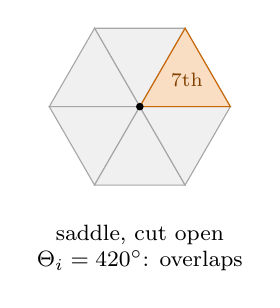
\begin{tikzpicture}[scale=1.15]
  \foreach \k in {0,...,5} {\filldraw[draw=gray!70, fill=gray!12] (0,0) -- ({60*\k}:1) -- ({60*(\k+1)}:1) -- cycle;}
  \filldraw[draw=orange!80!black, fill=orange!35, fill opacity=0.6] (0,0) -- (0:1) -- (60:1) -- cycle;
  \node[orange!50!black, font=\scriptsize, align=center] at (30:0.6) {7th};
  \fill (0,0) circle (1.2pt);
  \node[below, font=\footnotesize, align=center] at (0,-1.2) {saddle, cut open\\$\Theta_i = 420^\circ$: overlaps};
\end{tikzpicture}\hfill
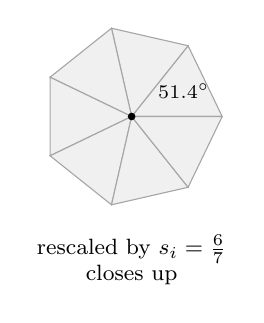
\begin{tikzpicture}[scale=1.15]
  \foreach \k in {0,...,6} {\filldraw[draw=gray!70, fill=gray!12] (0,0) -- ({360/7*\k}:1) -- ({360/7*(\k+1)}:1) -- cycle;}
  \node[font=\scriptsize] at ({180/7}:0.64) {$51.4^\circ$};
  \fill (0,0) circle (1.2pt);
  \node[below, font=\footnotesize, align=center] at (0,-1.2) {rescaled by $s_i = \frac{6}{7}$\\closes up};
\end{tikzpicture}
}
\caption{The faces around a vertex, cut along the reference edge (blue, $\theta = 0$) and flattened. Five equilateral triangles: $\Theta_i = 300^\circ$, a gap of $60^\circ$, the angle defect. Rescaling every angle by $s_i = 2\pi/\Theta_i = 6/5$ closes the gap: every $60^\circ$ corner becomes $72^\circ$. Seven equilateral triangles: $\Theta_i = 420^\circ$, the seventh overlaps the first; rescaling by $6/7$ turns every corner into $51.4^\circ$.}
\label{fig:cone_rescale}
\end{figure}

\paragraph{The angle defect is a curvature.} The ant cannot see its surface bend in space. What it can do is carry an arrow around a closed loop, keeping the arrow parallel at every step, and look at it when it comes back. On a plane the arrow comes back as it left. On a curved surface it comes back turned, and the angle of the turn, the \emph{holonomy} of the loop, is the total Gaussian curvature $\int K\, dA$ of the region enclosed by the loop, by~(\ref{eqn:r3_holonomy})~[\,$\psi_{\text{end}} = e^{\mathsf T\int K\,dA}\psi_{\text{start}}$\,].

Let us compute that rotation for a small loop around the vertex $i$ of a mesh. Inside a face the arrow does not change, because the face is flat; across an edge it is unfolded. After flattening the fan, both steps say the same thing: in the plane of the fan, the arrow keeps its direction. Suppose it starts in the first face at the angle $u$ from the reference edge $e_0$. It goes around through all the faces of the fan, always pointing the same way in the plane. When it reaches the end of the fan, the edge there is the second copy of $e_0$, which lies at the angle $\Theta_i$ from the first copy; relative to that second copy the arrow makes the angle $u - \Theta_i$. But the second copy of $e_0$ is $e_0$ itself on the surface: the loop is closed. So the arrow is back in the first face at the angle $u - \Theta_i$, which we rewrite by adding and subtracting $2\pi$:
\begin{align*}
u - \Theta_i &= u + 2\pi - \Theta_i - 2\pi && \text{(add $2\pi - 2\pi = 0$)} \\
&= u + (2\pi - \Theta_i) - 2\pi && \text{(group)} \\
&= u + \kappa_i - 2\pi && \text{(\ref{eqn:defect})~[\,$\kappa_i = 2\pi - \Theta_i$\,].}
\end{align*}
Subtracting a full turn $2\pi$ does not change a direction, so the arrow points at $u + \kappa_i$: it has turned by the angle defect $\kappa_i$. The loop can be as small as we like, as long as it goes around $i$, and the turn is always $\kappa_i$; a loop that does not go around a vertex stays in flat faces and does not turn at all. So all the curvature of the mesh sits at its vertices, and $\kappa_i$ is the total curvature $\int K\, dA$ of the neighborhood of $i$, concentrated at the vertex \cite{Sharp2019}. In gauge language: the faces are flat gauges glued to one another across the edges by the unfoldings, and the product of these transitions around the vertex is $e^{\mathsf T\kappa_i}$, the discrete form of the holonomy~(\ref{eqn:r3_holonomy}). The field strength is zero in every face and concentrated at the vertex. It is a sum of angles of triangles, which are functions of the edge lengths, so it is intrinsic.

\paragraph{The defects add up to $2\pi\chi$.} On a smooth closed surface, the total curvature $\int K\, dA$ is $2\pi \chi$, where $\chi$ is the \emph{Euler characteristic}, $2$ for any surface shaped like a sphere (the Gauss--Bonnet theorem). On a mesh, $\chi = V - E + F$, the number of vertices minus the number of edges plus the number of faces. We show that $\sum_i \kappa_i = 2\pi (V - E + F)$ for a closed mesh in three steps.

\emph{Step 1: the angles.} Every corner of every triangle belongs to exactly one vertex. So the sum of all the total angles, $\sum_i \Theta_i$, is the sum of all the corners of all the triangles, which we can add up triangle by triangle instead of vertex by vertex. Each triangle contributes the sum of its three angles, $\pi$, so $\sum_i \Theta_i = \pi F$.

\emph{Step 2: the edges.} Count the pairs (edge, triangle containing it). Each triangle has three edges, so there are $3F$ pairs; on a closed mesh each edge lies in exactly two triangles, so there are $2E$ pairs. Hence $2E = 3F$, that is, $E = \frac32 F$.

\emph{Step 3: the sum.} By~(\ref{eqn:defect})~[\,$\kappa_i = 2\pi - \Theta_i$\,],
\begin{align*}
\sum_i \kappa_i &= \sum_i (2\pi - \Theta_i) && \text{(substitute)} \\
&= 2\pi V - \sum_i \Theta_i && \text{($V$ vertices, each contributing $2\pi$)} \\
&= 2\pi V - (\pi F) && \text{(Step 1)} \\
&= 2\pi V - 2\pi \big(\tfrac32 F - F\big) && \text{($\pi F = 2\pi \cdot \tfrac12 F$ and $\tfrac12 = \tfrac32 - 1$)} \\
&= 2\pi V - 2\pi \big(E - F\big) && \text{(Step 2, $\tfrac32F = E$)} \\
&= 2\pi (V - E + F) = 2\pi\chi && \text{(distribute).}
\end{align*}
For the icosahedron, $V - E + F = 12 - 30 + 20 = 2$; every vertex has five equilateral triangles, $\Theta_i = 5 \cdot 60^\circ = 300^\circ$ and $\kappa_i = 60^\circ$, and the twelve defects add up to $12 \cdot 60^\circ = 720^\circ = 4\pi = 2\pi \cdot 2$. On a mesh with boundary the same count works with $\pi - \Theta_i$ at the boundary vertices.

The program checks this on the cactus. The function \code{totalCurvature} of \code{ga\_fem.cpp} adds $2\pi - \Theta_i$ over the interior vertices and $\pi - \Theta_i$ over the boundary vertices (line 476), with $\Theta_i$ taken from the walk around each vertex that we describe below:
\lstinputlisting[firstline=474, lastline=478, firstnumber=474]{../src/ga_fem.cpp}
The angle defects of the cactus add up to $12.566371 = 4\pi$, the value of a sphere, and the program prints $2\pi(V - E + F) = 12.566371$ next to it.

\subsection{Why a vertex has no tangent plane}

At a point $p$ of a smooth surface, the directions in which one can leave $p$ form a full circle, a turn of $2\pi$: a small circle of radius $r$ around $p$, drawn on the surface, has a length closer and closer to $2\pi r$ as $r \to 0$. The tangent vectors at $p$ are the vectors of the tangent plane: they can be added and multiplied by numbers, and the angle between two of them is an angle of the plane.

That is exactly what the finite element method needs at a vertex. The unknown at the vertex $i$ is a tangent vector, and the trial field~(\ref{eqn:ga_trial})~[\,$\psi_f = \sum_{i \in f} \phi_i\, e^{\mathsf T_f\rho_i^f}\psi_i$\,] combines the vectors of the three vertices of a face linearly, so $\psi_i$ must be a vector of some plane, with lengths and angles.

At a vertex of a mesh, the neighborhood of $i$ is exactly the cone of Figure~\ref{fig:cone_rescale}, at every magnification. A small circle of radius $r$ around $i$ crosses the faces one after another, as an arc of angle $\alpha_{i,f}$ and length $\alpha_{i,f}\, r$ in each face, so its length is
\begin{equation*}
\sum_{f\ni i}\alpha_{i,f}\, r = \Big(\sum_{f\ni i}\alpha_{i,f}\Big) r = \Theta_i\, r ,
\end{equation*}
not $2\pi r$. So when $\Theta_i \neq 2\pi$ the directions at $i$ form a circle of total angle $\Theta_i$, while the directions of any plane form a circle of total angle $2\pi$. Any way of identifying the directions at $i$ with the directions of a plane must change some angles. The gauge language says the same: a chart around $i$ that were an isometry, $G = I$, with a constant frame, would be a flat gauge, $\Omega = 0$, and by~(\ref{eqn:r3_holonomy}) a loop around $i$ would have no holonomy; but it has $\kappa_i$. So a flat chart at a curved vertex must distort the metric somewhere, and how it distorts is a choice of displacement gauge, a modeling decision. Part~\ref{part:matrix} made it with the vertex normal. Here we make it with the angles alone. When $\Theta_i = 2\pi$ the vertex does have a natural plane, the flattened fan, which closes exactly; a good choice should then give that plane.

\subsection{Directions at a vertex as angles}

The ant can describe a direction at the vertex by a single number: the angle it measures from a fixed edge. Choose a reference edge $e_0$ leaving the vertex: we take the same edge \code{vi.edge} whose projection is the vertex frame vector $t_i$ of Part~\ref{part:matrix} (in \code{computeGeometry} of \code{ga\_fem.cpp}, line 52 takes the direction of that edge, \code{vi.edge->pair->vertex->p - vi.p}, and line 53 projects it). Walk counterclockwise around the vertex, from one outgoing edge to the next, $e_0, e_1, e_2, \ldots$, and assign to each outgoing edge its \emph{cone angle}, the angle the ant measures from $e_0$:
\begin{equation}
\label{eqn:cone_angle}
\theta(e_0) = 0, \qquad \theta(e_{m+1}) = \theta(e_m) + \alpha_m ,
\end{equation}
where $\alpha_m$ is the angle at $i$ of the face between $e_m$ and $e_{m+1}$. Unrolling the recursion,
\begin{equation*}
\theta(e_1) = 0 + \alpha_0, \qquad \theta(e_2) = (\alpha_0) + \alpha_1, \qquad \ldots, \qquad \theta(e_m) = \alpha_0 + \alpha_1 + \cdots + \alpha_{m-1} .
\end{equation*}
Every direction at the vertex points into some corner and has a cone angle $\theta$ in $[0, \Theta_i)$: if it points into the corner between $e_m$ and $e_{m+1}$, at the angle $u$ from $e_m$ inside that face, its cone angle is $\theta(e_m) + u$. After a full turn, $\theta = \alpha_0 + \cdots + \alpha_{n-1} = \Theta_i$, which is again the direction of $e_0$. For the five equilateral triangles of Figure~\ref{fig:cone_rescale} the outgoing edges have the cone angles $0^\circ, 60^\circ, 120^\circ, 180^\circ, 240^\circ$, and $300^\circ$ is $e_0$ again.

To compute~(\ref{eqn:cone_angle}) the program must walk around each vertex in the half-edge structure. Its conventions decide the direction of the walk and the signs of the angles, so we describe them carefully.

\paragraph{Half edges.} The structure of \code{src/HalfEdge} stores each edge of the mesh as two \emph{half edges} of opposite directions, \code{e} and \code{e->pair}. A half edge has an origin, \code{e->vertex}, the vertex it leaves (\code{Mesh::addEdge} sets \code{e->vertex} to the first vertex $i$ of the edge from $i$ to $j$), and a face, \code{e->face}, the face that lies to its \emph{left}. The faces of the mesh are listed with their vertices in counterclockwise order, seen from the side towards which the face normal points; going from a half edge of a face to \code{e->next} goes around that face counterclockwise, and for a counterclockwise face the inside is always on the left, so all three half edges of a face have it on their left. At the boundary of the mesh, a half edge with nothing on its left has \code{e->face} equal to null.

\paragraph{Turning around a vertex.} Let \code{e} be a half edge leaving the vertex $v$, towards a neighbor $w$ (Figure~\ref{fig:t3_halfedge}). Its pair \code{e->pair} goes back from $w$ to $v$. The face to the left of \code{e->pair} is the face to the \emph{right} of \code{e}. In that face, the half edge after \code{e->pair} starts where \code{e->pair} ends, at $v$: so \code{e->pair->next} is again a half edge leaving $v$, the one on the other side of the face to the right of \code{e}. It is the next outgoing half edge \emph{clockwise}. This is the step of the iterator \code{Vertex::EdgeAroundIterator} of \code{HalfEdge/Vertex.h}, \code{run = run->pair->next}, so the natural walk around a vertex in this structure is clockwise, and the comment of \code{IntrinsicConnection.h} (lines 7 and 8) states the same convention.
\begin{figure}[t]
\centering
\begin{tikzpicture}[scale=1.5, >=Stealth]
  \coordinate (v) at (0,0);
  \coordinate (w) at (2.2,0);
  \coordinate (a) at ({2*cos(75)},{2*sin(75)});
  \coordinate (b) at ({2*cos(-75)},{2*sin(-75)});
  \fill[blue!8] (v) -- (w) -- (a) -- cycle;
  \fill[red!8] (v) -- (b) -- (w) -- cycle;
  \draw[thick,->] (v) -- (w);
  \node[above] at (1.4,0.02) {\code{e}};
  \draw[thick,->] ([yshift=-4pt]w) -- ([yshift=-4pt]v);
  \node[below] at (1.45,-0.1) {\code{e->pair}};
  \draw[thick,->] (v) -- (b);
  \node[left] at ($(v)!0.75!(b)$) {\code{e->pair->next}};
  \draw[->, gray] (v) -- (a);
  \node[left, gray] at ($(v)!0.75!(a)$) {next counterclockwise};
  \draw[gray] (w) -- (a) (b) -- (w);
  \node at (0.95,0.75) {\code{e->face}};
  \node at (1.0,-0.7) {\code{e->pair->face}};
  \fill (v) circle (1.5pt) node[left] {$v$};
  \fill (w) circle (1.5pt) node[right] {$w$};
  \draw[->, thick, orange] (0.55,0) arc (0:-75:0.55);
  \node[orange] at (0.62,-0.38) {$\alpha$};
\end{tikzpicture}
\caption{The half edges around a vertex $v$. The face of a half edge lies to its left. \code{e->pair} runs from $w$ back to $v$, with the face to the right of \code{e} on its left; the next half edge of that face, \code{e->pair->next}, leaves $v$ again, clockwise from \code{e}. The corner between them, of angle $\alpha$, belongs to the face to the left of \code{e->pair->next}, and is its corner at its origin.}
\label{fig:t3_halfedge}
\end{figure}

\paragraph{Which corner lies between two steps.} When the walk goes from \code{e} to \code{next = e->pair->next}, it crosses one corner at $v$: that of the face to the right of \code{e}, which is the face to the left of \code{next}. Counterclockwise, that corner starts at \code{next} and ends at \code{e}. Its angle is the angle of the face of \code{next} at the origin of \code{next}. The small helper \code{angleAtOrigin} returns exactly this: it finds the position \code{a} of the half edge among the three half edges of its face, so that the half edge goes from \code{v[a]} to \code{v[a+1]}, and returns \code{angle[a]}, the corner angle at \code{v[a]}, its origin:
\lstinputlisting[firstline=96, lastline=103, firstnumber=96]{../src/IntrinsicConnection.h}

\paragraph{Clockwise walk, negative angles.} Because the walk is clockwise, the program builds~(\ref{eqn:cone_angle}) backwards: it starts at $e_0$ with $\theta = 0$ and \emph{subtracts} the angle of each corner it crosses. In the counterclockwise numbering $e_0, e_1, \ldots, e_{n-1}$, the first step goes from $e_0$ to $e_{n-1}$ across the corner $\alpha_{n-1}$, and the program gives $e_{n-1}$ the angle $-\alpha_{n-1}$. By~(\ref{eqn:cone_angle}) the counterclockwise angle of $e_{n-1}$ is $\alpha_0 + \cdots + \alpha_{n-2} = \Theta_i - \alpha_{n-1}$. The next step gives $e_{n-2}$ the angle $-\alpha_{n-1} - \alpha_{n-2}$, while~(\ref{eqn:cone_angle}) gives $\Theta_i - \alpha_{n-1} - \alpha_{n-2}$, and so on. Every edge other than $e_0$ gets
\begin{equation*}
\begin{aligned}
\theta_{\text{code}}(e_m) &= -(\alpha_m + \cdots + \alpha_{n-1}) \\
&= (\alpha_0 + \cdots + \alpha_{m-1}) - (\alpha_0 + \cdots + \alpha_{n-1}) \\
&= \theta(e_m) - \Theta_i , \qquad m = 1, \ldots, n-1,
\end{aligned}
\end{equation*}
an angle in $(-\Theta_i, 0)$, and $e_0$ keeps $0$. For the five equilateral triangles the program stores $0^\circ, -240^\circ, -180^\circ, -120^\circ, -60^\circ$ for $e_0, \ldots, e_4$, which are $0^\circ, 60^\circ, 120^\circ, 180^\circ, 240^\circ$ minus $300^\circ$. Each corner still spans $[\theta, \theta + \alpha]$ from its counterclockwise first edge; for instance the corner between $e_4$ and $e_0$ spans $[-60^\circ, 0^\circ]$. Both descriptions differ by a shift of $\Theta_i$, the angle of a full turn around the vertex: the same direction, as $u$ and $u - \Theta_i$ were in the holonomy computation above. We shall see after the rescaling that the shift becomes exactly $2\pi$, and disappears from every formula of the method.

\paragraph{Boundary vertices.} At a boundary vertex the faces do not go all the way around. \code{Mesh::linkBoundary} sets the reference half edge \code{vi.edge} of such a vertex to the outgoing boundary half edge, the one with no face on its left: the outside of the mesh lies on its left and all the faces lie clockwise from it. The clockwise walk from it therefore visits every corner, and it stops when it reaches the last outgoing half edge, the one whose \code{pair} has no face, because there is nothing clockwise beyond it. The cone angles are then measured clockwise from the boundary edge and are negative, in $[-\Theta_i, 0]$. There is no full turn, so there is nothing to shift.

\subsection{The stretched cone}

The cone angles give every direction at the vertex a number, but on a circle of total angle $\Theta_i$, not $2\pi$. To make a plane we stretch the cone so that it closes. Define the \emph{scale} of the vertex and the \emph{angle} of a direction in the plane of the vertex,
\begin{equation}
\label{eqn:scale}
s_i = \frac{2\pi}{\Theta_i}, \qquad \varphi = s_i\, \theta .
\end{equation}
As $\theta$ runs over $[0, \Theta_i)$, $\varphi$ runs over $[s_i\cdot 0, s_i\Theta_i) = [0, \frac{2\pi}{\Theta_i}\Theta_i) = [0, 2\pi)$: a full turn. This is our tangent plane of the vertex: a plane whose directions are the angles $\varphi$, with $\varphi = 0$ along the reference edge. A tangent vector at $i$ is a length and an angle $\varphi$, that is, the complex number $\psi = |U|\, e^{\mathsf T \varphi}$ of Part~\ref{part:ga}, the spinor coordinate of $U$ in the frame of the reference edge.

Picture the stretching as a map of the whole fan onto the plane. A point of the fan at the distance $r$ from the vertex and at the cone angle $\theta$ goes to the point of the plane with the polar coordinates $r$ and $s_i\theta$. Each edge leaving the vertex goes to a ray; each corner from $\theta_e$ to $\theta_e + \alpha$ goes to the sector from $s_i\theta_e$ to $s_i(\theta_e + \alpha) = s_i\theta_e + s_i\alpha$, of angle $s_i\alpha$; a circle of radius $r$ around the vertex, of length $\Theta_i r$ on the cone, goes to the circle of radius $r$ and length $2\pi r$ in the plane. The stretching multiplies every angle at the vertex by the same factor $s_i$, so the corners tile the plane without gap or overlap (Figure~\ref{fig:cone_rescale}).

\paragraph{The vertex chart.} This stretched plane is the flat chart of the vertex, in the sense of Section~\ref{section:r3_idea}, and its frame is the constant direction $\varphi = 0$, the reference edge. The map from the cone to the plane, $(r, \theta) \mapsto (r, s_i\theta)$, is its displacement gauge, read backwards; it keeps distances from the vertex and multiplies the angles at the vertex by $s_i$, so it is not an isometry when $s_i \ne 1$, as the previous subsection said it could not be. The distortion costs nothing in the integrals, which are all done in the face charts; it shows only in how the vertex chart is connected to the face charts, which is Section~\ref{section:int_connection}.

\paragraph{Where the defect went.} The angle defect has not disappeared: it has been spread evenly over the corners. A corner of angle $\alpha_m$ becomes $s_i \alpha_m$, so it absorbs the share $s_i\alpha_m - \alpha_m = (s_i - 1)\, \alpha_m$ of the defect, in proportion to its angle. The shares add up to the defect:
\begin{align*}
\sum_m (s_i - 1)\,\alpha_m &= (s_i - 1)\sum_m \alpha_m && \text{(factor out)} \\
&= (s_i - 1)\,\Theta_i && \text{(\ref{eqn:total_angle})} \\
&= s_i\Theta_i - \Theta_i && \text{(distribute)} \\
&= \Big(\frac{2\pi}{\Theta_i}\Big)\Theta_i - \Theta_i && \text{(\ref{eqn:scale})} \\ &= 2\pi - \Theta_i = \kappa_i && \text{(\ref{eqn:defect}).}
\end{align*}
On a cone, $s_i > 1$ and the corners are widened to close the gap; at a saddle, $s_i < 1$ and they are narrowed to remove the overlap. On a fine mesh of a smooth surface $\Theta_i \to 2\pi$, $s_i \to 1$, and the stretching vanishes.

\paragraph{The negative angles of the code.} They are $\theta_{\text{code}} = \theta - \Theta_i$, so after the rescaling
\begin{equation*}
s_i\theta_{\text{code}} = s_i(\theta - \Theta_i) = s_i\theta - s_i\Theta_i = \varphi - 2\pi ,
\end{equation*}
exactly one full turn less: the same direction, and the same unit complex number, since $e^{\mathsf T(\varphi - 2\pi)} = e^{\mathsf T\varphi}e^{-\mathsf T 2\pi} = e^{\mathsf T\varphi}(\cos 2\pi - \mathsf T\sin 2\pi) = e^{\mathsf T\varphi}$. Every formula of the method uses angles only through such unit complex numbers, so the code can keep its negative angles.

\paragraph{Boundary vertices.} At a boundary vertex the directions do not form a circle but an arc, from the boundary edge on one side to the boundary edge on the other: there is no loop to close, and we do not rescale, $s_i = 1$. This keeps a flat sheet exactly flat: the corner of a rectangle keeps its angle $\pi/2$.

\paragraph{The code.} Here is the walk around every vertex, the total angle and the scale~(\ref{eqn:scale})~[\,$s_i = 2\pi/\Theta_i,\ \varphi = s_i\theta$\,], followed, on lines 125 to 138, by the connection of every corner, which we explain in Section~\ref{section:int_connection}:
\lstinputlisting[firstline=104, lastline=138, firstnumber=104]{../src/IntrinsicConnection.h}
Line by line, for lines 104 to 124:
\begin{itemize}
\item Line 107 starts at the reference half edge, $e = e_0$ = \code{vi.edge}, and lines 108 and 109 store $\theta(e_0) = 0$ in the map \code{outAngle}, which keeps the cone angle of every outgoing half edge.
\item Line 112 takes the pair of the current half edge. If it has no face (line 113), the walk has passed the last face of a boundary vertex: there is nothing clockwise beyond, and the loop ends with \code{boundary} set.
\item Line 114 is the clockwise step of Figure~\ref{fig:t3_halfedge}, \code{next = e->pair->next}.
\item Line 115 subtracts the angle of the corner just crossed, the corner of the face of \code{next} at its origin: this is~(\ref{eqn:cone_angle}) walked backwards.
\item Line 116 ends the loop when the walk is back at $e_0$, after crossing the last corner. At that point $\theta = -\Theta_i$. Otherwise line 117 stores the cone angle of \code{next}, and line 118 moves on.
\item Line 121 is the total angle~(\ref{eqn:total_angle})~[\,$\Theta_i = \sum_{f\ni i}\alpha_{i,f}$\,], $\Theta_i = -\theta$, the sum of all the corners crossed.
\item Line 122 records whether the vertex is on the boundary; the second test, \code{!vi.edge->face}, says the same as the first for the meshes built by \code{linkBoundary}, and is only a safeguard.
\item Line 123 is the scale~(\ref{eqn:scale}), $s_i = 2\pi/\Theta_i$ for an interior vertex and $1$ at the boundary.
\end{itemize}

\subsection{What the vertex normal does instead}

The vertex plane of Part~\ref{part:ga} solves the same problem in another way. Each face is rolled into the plane orthogonal to $n_i$ by the rotor $Q_{i \to f}$ of~(\ref{eqn:ga_Q})~[\,$Q_{i\to f} = \frac{1 + n_f n_i}{|1 + n_f n_i|}$\,], run backwards. A rotation preserves angles, so every corner keeps its true angle $\alpha_{i,f}$ in the vertex plane, and the rolled corners together cover $\Theta_i$, not $2\pi$. They cannot tile the plane: they leave gaps between neighbors when $\Theta_i < 2\pi$ and overlap when $\Theta_i > 2\pi$, and the gaps add up to the angle defect. Where the gaps fall depends on how each face is tilted with respect to the vertex normal, an extrinsic fact. The rescaling~(\ref{eqn:scale}) spreads the defect in proportion to the angles, an intrinsic fact. Even at a flat vertex, $\Theta_i = 2\pi$, the rolled corners fit edge to edge only if all the faces are rolled about one line, as along a straight fold; otherwise they leave gaps and overlaps that cancel in total but not one by one, which is what happens on the Miura-ori of Figure~\ref{fig:miura}. On a symmetric vertex the two planes agree; on any other they differ, as the next two examples show.

\paragraph{How to read the tables of the two examples.} Each row is one corner at the vertex, in counterclockwise order from the reference edge, and $\alpha$ is its angle. The two groups of columns say where each method puts that corner in its plane of the vertex, as a sector of directions. ``From'' is the angle, in the plane of the vertex, of the first edge of the corner (counterclockwise), measured from the reference direction; ``width'' is the angle of the sector. For the intrinsic plane, from $= s_i\,\theta_e$ and width $= s_i\, \alpha$, by~(\ref{eqn:scale}). For the extrinsic plane, ``from'' is the angle of the rolled first edge measured from $t_i$, and the width is $\alpha$ itself, since rolling keeps angles; ``gap'' is the empty angle between the end of this sector and the start of the next. So in the intrinsic columns each row ends where the next begins, while in the extrinsic columns from $+$ width $+$ gap gives the next ``from''. The program computes the columns with these lines of \code{workedExamplesIntrinsic} in \code{ga\_fem.cpp}:
\lstinputlisting[firstline=686, lastline=697, firstnumber=686]{../src/ga_fem.cpp}
The apex is the first vertex of every face of the pyramid, so its corner is \code{a = 0}, and \code{h[0]} is the first edge of the corner. Line 691 turns the code's negative cone angle back into the counterclockwise one of~(\ref{eqn:cone_angle}): adding $\Theta_i$ and reducing modulo $\Theta_i$ maps $(-\Theta_i, 0]$ onto $[0, \Theta_i)$, the shift of the previous subsection undone. The table prints $s_i$ times it as ``from''. Lines 693 to 695 are Part~\ref{part:ga}: line 693 rolls the first edge of the face into the plane of the vertex normal, with the smallest rotor from $n_f$ to $n_i$; line 694 measures its angle from $t_i$, counterclockwise about $n_i$, with \code{atan2} of the sine $(t_i \times d) \cdot n_i$ and the cosine $t_i \cdot d$; and line 695 brings the angle into $[0, 2\pi)$.

\begin{example}
\label{ex:int_pyramid}
The apex of a pyramid over a regular pentagon of radius $1$, at the height $h = 0.6180$ that makes the five faces equilateral. Each corner at the apex is $60^\circ$, so $\Theta_i = 5\cdot 60^\circ = 300^\circ$, $\kappa_i = 360^\circ - 300^\circ = 60^\circ$ and $s_i = 360/300 = 1.2$; the vertex normal is vertical, by symmetry. The program prints, for the corners in counterclockwise order from the reference edge:
\begin{center}
\footnotesize
\begin{tabular}{c c | c c | c c c}
\toprule
& & \multicolumn{2}{c|}{intrinsic} & \multicolumn{3}{c}{extrinsic (rolled)} \\
corner & $\alpha$ & from & width & from & width & gap \\
\midrule
0 & $60^\circ$ & $0^\circ$ & $72^\circ$ & $6^\circ$ & $60^\circ$ & $12^\circ$ \\
1 & $60^\circ$ & $72^\circ$ & $72^\circ$ & $78^\circ$ & $60^\circ$ & $12^\circ$ \\
$\vdots$ & & & & & & \\
4 & $60^\circ$ & $288^\circ$ & $72^\circ$ & $294^\circ$ & $60^\circ$ & $12^\circ$ \\
\bottomrule
\end{tabular}
\end{center}
The intrinsic plane stretches each corner from $60^\circ$ to $1.2 \times 60^\circ = 72^\circ$, and five of them make $5 \times 72^\circ = 360^\circ$. The extrinsic plane keeps each at $60^\circ$ and leaves five gaps of $12^\circ$, again $5\times 12^\circ = 60^\circ$ in total. Its first sector starts at $6^\circ$, not at $0^\circ$, because the reference direction $t_i$ is the projection of the reference edge onto the plane of the vertex, not its rolled image. The middle directions of the corners, their bisectors, are the same in both: intrinsic $0^\circ + 72^\circ/2 = 36^\circ$, extrinsic $6^\circ + 60^\circ/2 = 36^\circ$, and then $108^\circ, 180^\circ, \ldots$ Since the connection of the next section matches bisectors, the two connections are equal at this vertex; the program finds them equal to rounding ($2.5 \cdot 10^{-14}$ degrees).
\end{example}

\begin{example}
\label{ex:int_leaning}
Move the apex of Example~\ref{ex:int_pyramid} by $0.4$ towards one corner of the pentagon. The corners become $70.49^\circ$, $70.49^\circ$, $51.37^\circ$, $46.81^\circ$, $51.37^\circ$, with $\Theta_i = 290.53^\circ$, $\kappa_i = 69.47^\circ$ and $s_i = 360/290.53 = 1.2391$. The vertex normal is still vertical. The normal of the code averages the cross products $(x_k - x_i) \times (x_{k+1} - x_i)$ of the faces, where $x_k$ runs over the ring of neighbors (with $x_{k+1}$ the next one around). Each of them expands, by the distributive law, as
\begin{align*}
&(x_k - x_i) \times (x_{k+1} - x_i) \\
&\quad= x_k \times x_{k+1} - x_k \times x_i - x_i \times x_{k+1} + x_i \times x_i && \text{(distribute)} \\
&\quad= x_k \times x_{k+1} + x_i \times x_k - x_i \times x_{k+1} + 0 && \text{($a\times b = -b\times a$, $a \times a = 0$)} \\
&\quad= x_k \times x_{k+1} - x_i \times (x_{k+1} - x_k) && \text{(factor $x_i \times$).}
\end{align*}
Summed around the ring, the differences $x_{k+1} - x_k$ add up to zero (the sum telescopes and the ring is closed), so the terms with $x_i$ cancel: the sum does not depend on the apex at all, and equals twice the vector area of the pentagon, which is vertical. Figure~\ref{fig:pyramid} shows where each method puts the corners:
\begin{center}
\footnotesize
\begin{tabular}{c c | c c | c c c}
\toprule
& & \multicolumn{2}{c|}{intrinsic} & \multicolumn{3}{c}{extrinsic (rolled)} \\
corner & $\alpha$ & from & width & from & width & gap \\
\midrule
0 & $70.488^\circ$ & $0^\circ$ & $87.341^\circ$ & $13.146^\circ$ & $70.488^\circ$ & $23.662^\circ$ \\
1 & $70.488^\circ$ & $87.341^\circ$ & $87.341^\circ$ & $107.296^\circ$ & $70.488^\circ$ & $15.181^\circ$ \\
2 & $51.373^\circ$ & $174.682^\circ$ & $63.655^\circ$ & $192.964^\circ$ & $51.373^\circ$ & $7.720^\circ$ \\
3 & $46.814^\circ$ & $238.337^\circ$ & $58.007^\circ$ & $252.057^\circ$ & $46.814^\circ$ & $7.720^\circ$ \\
4 & $51.373^\circ$ & $296.345^\circ$ & $63.655^\circ$ & $306.592^\circ$ & $51.373^\circ$ & $15.181^\circ$ \\
\bottomrule
\end{tabular}
\end{center}
Read the first row: in the intrinsic plane the corner of $70.488^\circ$ becomes the sector from $0^\circ$ to $87.341^\circ = 1.2391 \times 70.488^\circ$, and the next corner starts exactly there. In the extrinsic plane it keeps its $70.488^\circ$, from $13.146^\circ$ to $13.146^\circ + 70.488^\circ = 83.634^\circ$, and the next corner starts $23.662^\circ$ later, at $83.634^\circ + 23.662^\circ = 107.296^\circ$.

Both spread the defect of $69.47^\circ$ over the five corners, but differently. The intrinsic plane gives each corner $(s_i - 1)\alpha$: $16.85^\circ$, $16.85^\circ$, $12.28^\circ$, $11.19^\circ$, $12.28^\circ$, in proportion to the angles. The extrinsic plane leaves gaps of $23.66^\circ$, $15.18^\circ$, $7.72^\circ$, $7.72^\circ$, $15.18^\circ$, which depend on the tilt of the faces: the largest gap opens between the two faces on the side towards which the apex leans, which are tilted most with respect to the vertex normal. The bisectors now differ: from $+$ half the width is $0^\circ + 87.341^\circ/2 = 43.67^\circ$ against $13.146^\circ + 70.488^\circ/2 = 48.39^\circ$ in the first row, and the five differences are $4.7^\circ, 11.5^\circ, 12.1^\circ, 8.1^\circ$ and $4.1^\circ$; so do the two connections, by up to $12.1^\circ$.
\end{example}
\begin{figure}[t]
\centering
\adjustbox{max width=\linewidth}{% generated by make_figures.py: the leaning pyramid of Worked example 5
\begin{tikzpicture}[scale=1.2]
\filldraw[draw=gray!70, fill=red!18] (0,0) -- (0.000:1) arc (0.000:70.488:1) -- cycle;
\node[font=\tiny] at (35.244:0.6) {$70.5^\circ$};
\filldraw[draw=gray!70, fill=orange!22] (0,0) -- (70.488:1) arc (70.488:140.975:1) -- cycle;
\node[font=\tiny] at (105.731:0.6) {$70.5^\circ$};
\filldraw[draw=gray!70, fill=yellow!30] (0,0) -- (140.975:1) arc (140.975:192.348:1) -- cycle;
\node[font=\tiny] at (166.661:0.6) {$51.4^\circ$};
\filldraw[draw=gray!70, fill=green!18] (0,0) -- (192.348:1) arc (192.348:239.162:1) -- cycle;
\node[font=\tiny] at (215.755:0.6) {$46.8^\circ$};
\filldraw[draw=gray!70, fill=blue!14] (0,0) -- (239.162:1) arc (239.162:290.534:1) -- cycle;
\node[font=\tiny] at (264.848:0.6) {$51.4^\circ$};
\draw[-{Stealth[length=1.6mm]}, thick, blue!70!black] (0,0) -- (0:1.2);
\fill (0,0) circle (1.2pt);
\node[below, font=\footnotesize, align=center] at (0,-1.35) {cut open and flattened:\\$\Theta_i = 290.5^\circ$, a gap of $69.5^\circ$};
\end{tikzpicture}
\hfill
\begin{tikzpicture}[scale=1.2]
\filldraw[draw=gray!70, fill=red!18] (0,0) -- (0.000:1) arc (0.000:87.341:1) -- cycle;
\node[font=\tiny] at (43.670:0.6) {$87.3^\circ$};
\filldraw[draw=gray!70, fill=orange!22] (0,0) -- (87.341:1) arc (87.341:174.682:1) -- cycle;
\node[font=\tiny] at (131.011:0.6) {$87.3^\circ$};
\filldraw[draw=gray!70, fill=yellow!30] (0,0) -- (174.682:1) arc (174.682:238.337:1) -- cycle;
\node[font=\tiny] at (206.509:0.6) {$63.7^\circ$};
\filldraw[draw=gray!70, fill=green!18] (0,0) -- (238.337:1) arc (238.337:296.345:1) -- cycle;
\node[font=\tiny] at (267.341:0.6) {$58.0^\circ$};
\filldraw[draw=gray!70, fill=blue!14] (0,0) -- (296.345:1) arc (296.345:360.000:1) -- cycle;
\node[font=\tiny] at (328.172:0.6) {$63.7^\circ$};
\draw[-{Stealth[length=1.6mm]}, thick, blue!70!black] (0,0) -- (0:1.2);
\fill (0,0) circle (1.2pt);
\node[below, font=\footnotesize, align=center] at (0,-1.35) {intrinsic: every corner\\stretched by $s_i = 1.2391$};
\end{tikzpicture}
\hfill
\begin{tikzpicture}[scale=1.2]
\filldraw[draw=gray!70, fill=red!18] (0,0) -- (13.146:1) arc (13.146:83.634:1) -- cycle;
\node[font=\tiny] at (48.390:0.6) {$70.5^\circ$};
\fill[red!55] (0,0) -- (83.634:1.12) arc (83.634:107.296:1.12) -- cycle;
\node[red!60!black, font=\tiny] at (95.465:1.3) {$23.7^\circ$};
\filldraw[draw=gray!70, fill=orange!22] (0,0) -- (107.296:1) arc (107.296:177.783:1) -- cycle;
\node[font=\tiny] at (142.539:0.6) {$70.5^\circ$};
\fill[red!55] (0,0) -- (177.783:1.12) arc (177.783:192.964:1.12) -- cycle;
\node[red!60!black, font=\tiny] at (185.374:1.3) {$15.2^\circ$};
\filldraw[draw=gray!70, fill=yellow!30] (0,0) -- (192.964:1) arc (192.964:244.337:1) -- cycle;
\node[font=\tiny] at (218.651:0.6) {$51.4^\circ$};
\fill[red!55] (0,0) -- (244.337:1.12) arc (244.337:252.057:1.12) -- cycle;
\node[red!60!black, font=\tiny] at (248.197:1.3) {$7.7^\circ$};
\filldraw[draw=gray!70, fill=green!18] (0,0) -- (252.057:1) arc (252.057:298.872:1) -- cycle;
\node[font=\tiny] at (275.465:0.6) {$46.8^\circ$};
\fill[red!55] (0,0) -- (298.872:1.12) arc (298.872:306.592:1.12) -- cycle;
\node[red!60!black, font=\tiny] at (302.732:1.3) {$7.7^\circ$};
\filldraw[draw=gray!70, fill=blue!14] (0,0) -- (306.592:1) arc (306.592:357.965:1) -- cycle;
\node[font=\tiny] at (332.278:0.6) {$51.4^\circ$};
\fill[red!55] (0,0) -- (357.965:1.12) arc (357.965:373.146:1.12) -- cycle;
\node[red!60!black, font=\tiny] at (365.555:1.3) {$15.2^\circ$};
\draw[-{Stealth[length=1.6mm]}, thick, blue!70!black] (0,0) -- (0:1.2);
\fill (0,0) circle (1.2pt);
\node[below, font=\footnotesize, align=center] at (0,-1.35) {extrinsic: every corner rolled\\rigidly, gaps in red};
\end{tikzpicture}
}
\caption{The leaning pyramid of Example~\ref{ex:int_leaning}, seen from its apex, corners counterclockwise from the reference edge (blue). Left: cut open and flattened, with a gap of $69.5^\circ$, the angle defect. Middle: the intrinsic vertex plane, every corner stretched by the same factor. Right: the extrinsic vertex plane of Part~\ref{part:ga}, every corner rolled rigidly into the plane orthogonal to the vertex normal; the defect falls into the gaps between them (red), unevenly.}
\label{fig:pyramid}
\end{figure}

%%% ----------------------------------------------------------------------
\section{Stage 5, the Gauge Transitions: from a Vertex Chart into a Face Chart}
\label{section:int_connection}

We now have a flat chart at every vertex, made from the angles, and a flat chart in every face, the layout with the frame along its $x$ axis. The finite element method needs one more thing, the third ingredient of Stage 4: for each corner, the transition~(\ref{eqn:r3_transition})~[\,$\psi_B = e^{-\mathsf T\theta_{AB}}\psi_A$\,] that converts the coordinate of a vector in the chart of the vertex into its coordinate in the chart of the face. In the smooth theory it would be the parallel transport~(\ref{eqn:r3_transport})~[\,$\psi(s) = e^{-\mathsf T\int_0^s\omega}\psi(0)$\,] along the short way from the vertex into the face, combined with the change of frame; on the mesh it must be chosen, and the choice carries the curvature. With it, Stage 5 ends with the finite element space (Section~\ref{section:r3_space}).

\subsection{What the finite element method needs}

The element matrix~(\ref{eqn:ga_element})~[\,$\mathrm L^f_{ij} = A_f(\nabla\phi_i\cdot\nabla\phi_j)\, e^{\mathsf T(\rho_j^f - \rho_i^f)}$\,] uses, for each corner of a face, a unit complex number $e^{\mathsf T \rho_i^f}$ with the meaning of~(\ref{eqn:ga_connection})~[\,$e^{\mathsf T_f\rho_i^f} = t_f\,(Q t_i\widetilde Q)$\,]: a vector of angle $\varphi$ in the plane of vertex $i$ is the vector of angle $\varphi + \rho_i^f$ in the face frame. In words, $\rho_i^f$ is where the reference direction of the vertex, $\varphi = 0$, lands in the face. In spinor coordinates, the transport from the vertex into the face is the multiplication
\begin{equation*}
\psi = |\psi|\,e^{\mathsf T\varphi} \;\longmapsto\; e^{\mathsf T \rho_i^f}\psi = |\psi|\,e^{\mathsf T \rho_i^f}e^{\mathsf T\varphi} = |\psi|\,e^{\mathsf T(\varphi + \rho_i^f)} ,
\end{equation*}
a \emph{rotation} of the plane by $\rho_i^f$ (the exponents add because $\mathsf T$ commutes with itself).

It must be a rotation, and not some other map of directions, for this reason. The trial field~(\ref{eqn:ga_trial})~[\,$\psi_f = \sum_{i \in f} \phi_i\, e^{\mathsf T_f\rho_i^f}\psi_i$\,] builds the field in the face from the vectors of the three vertices, each carried into the face by its connection. At the vertex $i$ itself, where $\phi_i = 1$ and the other two hats vanish, the field is $e^{\mathsf T\rho_i^f}\psi_i$, and this must be the vector $\psi_i$ of the vertex, with the same length. And the mass and the stiffness integrate inner products $\langle\psi\widetilde\chi\rangle$ of such vectors over the face: if two vectors at the vertex make an angle $\delta$, their images in the face must make the same angle $\delta$, or the inner products measured in the face would not be those of the vertex. The maps of the plane that keep all lengths and all angles, and do not reflect, are exactly the rotations, the multiplications by unit complex numbers. So the connection of a corner is a single angle $\rho_i^f$. In gauge language: the transitions between charts must belong to the gauge group, the rotations $e^{\mathsf T\rho}$, because those are the changes of frame that leave the densities~(\ref{eqn:r3_density}) of the weak form unchanged (Section~\ref{section:r3_covariance}).

\subsection{The exact correspondence is not a rotation}

What angle? Let us first see what the stretched cone itself says. Look at one corner of the face $f$ at the vertex $i$. Let $e$ be the first edge of the corner in the counterclockwise order, with cone angle $\theta_e$ at the vertex and angle $\beta_e$ in the face frame; let $\alpha$ be the angle of the corner. A direction inside the corner that makes the angle $u \in [0, \alpha]$ with $e$ has
\begin{equation*}
\text{in the face:}\quad \beta = \beta_e + u, \qquad \text{at the vertex:}\quad \varphi = s_i (\theta_e + u),
\end{equation*}
the first because the face is flat and angles in it simply add, the second by~(\ref{eqn:scale})~[\,$\varphi = s_i\theta$\,], since the cone angle of the direction is $\theta = \theta_e + u$. The rotation that would carry this vertex direction to this face direction is the difference, which we expand and regroup:
\begin{align*}
\beta - \varphi &= (\beta_e + u) - \big(s_i (\theta_e + u)\big) && \text{(substitute)} \\
&= \beta_e + u - s_i\theta_e - s_i u && \text{(distribute $s_i$ and the minus sign)} \\
&= (\beta_e - s_i \theta_e) + (1 - s_i)\, u && \text{(group the terms with $u$).}
\end{align*}
It changes across the corner, by $(1 - s_i)\, \alpha$ from $u = 0$ to $u = \alpha$, unless $s_i = 1$. The exact correspondence stretches the corner, because the vertex plane is stretched and the face is not; it is not a rotation. For the corner of Figure~\ref{fig:corner_map}, with $\theta_e = 60^\circ$, $\alpha = 60^\circ$, $s_i = 1.2$ and $\beta_e = 0$, the constant is $\beta_e - s_i\theta_e = 0 - 1.2\cdot 60^\circ = -72^\circ$ and the slope is $1 - s_i = -0.2$; the difference is $-72^\circ$ along the first edge ($u = 0$), $-72^\circ - 0.2\cdot 30^\circ = -78^\circ$ in the middle and $-72^\circ - 0.2 \cdot 60^\circ = -84^\circ$ along the second edge ($u = 60^\circ$). We need a single number $\rho_i^f$ for the corner, and no single number is right for every direction.

\subsection{The best rotation: match the bisectors}

When no single number fits a whole range of values, we choose the number closest to all of them on average, in the sense of least squares: the one that makes the average of the squared mismatch as small as possible. Here the values are the exact rotations $\beta - \varphi$ of the directions of the corner, one for each $u \in [0, \alpha]$, and ``on average'' means the integral over $u$, in which each direction of the corner counts equally.

\emph{Step 1: name the constants.} Write the exact rotation as a linear function of $u$,
\begin{equation*}
m(u) = c + k\, u, \qquad c = \beta_e - s_i\theta_e, \qquad k = 1 - s_i ,
\end{equation*}
with $c$ its value along the first edge and $k$ its slope. The quantity to minimize over $\rho$ is
\begin{equation*}
E(\rho) = \int_0^\alpha \big(\rho - m(u)\big)^2\, du = \int_0^\alpha \big(\rho - (c + k u)\big)^2\, du .
\end{equation*}

\emph{Step 2: expand the integral.} Expand the square, $(\rho - m)^2 = \rho^2 - 2\rho\, m + m^2$, and split the integral into three:
\begin{align*}
E(\rho) &= \int_0^\alpha \big(\rho^2 - 2\rho\, m(u) + m(u)^2\big)\, du && \text{(expand the square)} \\
&= \int_0^\alpha \rho^2\, du - \int_0^\alpha 2\rho\, m(u)\, du + \int_0^\alpha m(u)^2\, du && \text{(the integral of a sum)} \\
&= \rho^2 \int_0^\alpha du - 2\rho \int_0^\alpha m(u)\, du + \int_0^\alpha m(u)^2\, du && \text{($\rho$ does not depend on $u$)} \\
&= \alpha\, \rho^2 - 2\rho\, b + C, && \text{($\textstyle\int_0^\alpha du = \alpha$)}
\end{align*}
where we named the two numbers that do not depend on $\rho$:
\begin{equation*}
b = \int_0^\alpha m(u)\, du, \qquad C = \int_0^\alpha m(u)^2\, du .
\end{equation*}
So $E$ is a quadratic polynomial in $\rho$ with the positive leading coefficient $\alpha$: a parabola opening upwards, smallest where its derivative vanishes.

\emph{Step 3: the derivative, set to zero.} Differentiate term by term with respect to $\rho$:
\begin{equation*}
\frac{dE}{d\rho} = \frac{d}{d\rho}(\alpha\rho^2) - \frac{d}{d\rho}(2b\rho) + \frac{d}{d\rho}C = 2\alpha\,\rho - 2b + 0 .
\end{equation*}
Setting it to zero and solving for $\rho$, one operation per line:
\begin{align*}
2\alpha\,\rho - 2b &= 0 \\
2\alpha\,\rho &= 2b && \text{(add $2b$)} \\
\rho &= \frac{b}{\alpha} = \frac{1}{\alpha} \int_0^\alpha m(u)\, du && \text{(divide by $2\alpha$; substitute $b$).}
\end{align*}
The second derivative is $2\alpha > 0$, so this is the minimum. It is the \emph{average} of the exact rotations over the corner: the constant closest, in least squares, to a function is its mean.

\emph{Step 4: the mean of the linear function.} Substitute $m(u) = c + ku$ into $b$:
\begin{align*}
b &= \int_0^\alpha (c + k u)\, du && \text{(substitute $m$)} \\
&= c\int_0^\alpha du + k\int_0^\alpha u\, du && \text{(split; constants out)} \\
&= c\,\alpha + k\,\frac{\alpha^2}{2} && \text{($\textstyle\int_0^\alpha u\,du = \big[\tfrac{u^2}2\big]_0^\alpha = \tfrac{\alpha^2}{2}$),}
\end{align*}
and divide by $\alpha$:
\begin{equation*}
\rho = \frac{1}{\alpha}\Big(c\,\alpha + k\,\frac{\alpha^2}{2}\Big) = c + k\,\frac{\alpha}{2} = m\Big(\frac\alpha2\Big) ,
\end{equation*}
the value of $m$ at the middle of the interval, $u = \alpha/2$. The mean of a linear function is its value at the midpoint.

\emph{Step 5: substitute back.} Put $c = \beta_e - s_i\theta_e$ and $k = 1 - s_i$ into $\rho = c + k\frac\alpha2$:
\begin{align*}
\rho &= \big(\beta_e - s_i\theta_e\big) + \big(1 - s_i\big)\frac\alpha2 && \text{(substitute $c$ and $k$)} \\
&= \beta_e - s_i\theta_e + \frac\alpha2 - s_i\frac\alpha2 && \text{(distribute $\tfrac\alpha2$)} \\
&= \Big(\beta_e + \frac\alpha2\Big) - \Big(s_i\theta_e + s_i\frac\alpha2\Big) && \text{(regroup: terms without $s_i$, terms with $s_i$)} \\
&= \Big(\beta_e + \frac\alpha2\Big) - s_i\Big(\theta_e + \frac\alpha2\Big) && \text{(factor $s_i$).}
\end{align*}
This is the connection of the corner:
\begin{equation}
\label{eqn:intrinsic_rho}
\rho_i^f = \Big(\beta_e + \frac{\alpha}{2}\Big) - s_i \Big(\theta_e + \frac{\alpha}{2}\Big).
\end{equation}

\emph{What it means.} The direction at the middle of the corner, $u = \alpha/2$, is its \emph{bisector}. The first bracket, $\beta_e + \frac\alpha2$, is the angle of the bisector in the face frame, and the second, $s_i(\theta_e + \frac\alpha2)$, is $s_i$ times its cone angle, the angle of the bisector in the plane of the vertex. So $\rho_i^f$ is the rotation that carries the bisector of the corner in the vertex plane exactly onto the bisector of the corner in the face: the intrinsic connection \emph{matches the bisectors}. Every other direction of the corner is carried with the error
\begin{equation*}
\rho - m(u) = \Big(c + k\frac\alpha2\Big) - \big(c + ku\big) = -k\Big(u - \frac\alpha2\Big) = (s_i - 1)\Big(u - \frac\alpha2\Big),
\end{equation*}
zero at the bisector and largest at the two edges, $u = 0$ and $u = \alpha$, where it is $\mp (s_i - 1)\alpha/2$: half the stretching on each side (Figure~\ref{fig:corner_map}).

For a flat vertex, $s_i = 1$, (\ref{eqn:intrinsic_rho}) becomes
\begin{equation*}
\rho_i^f = \Big(\beta_e + \frac\alpha2\Big) - (1)\Big(\theta_e + \frac\alpha2\Big) = \beta_e - \theta_e ,
\end{equation*}
with no mismatch at all: $k = 1 - 1 = 0$, the exact rotation $m(u) = c$ is the same for every direction, and the least-squares fit is exact. The vertex plane is then the plane of the flattened faces, and transport into each face is the exact unfolding. So on every part of a mesh that is intrinsically flat, however it is folded in space, the intrinsic connection is the exact parallel transport. This is why it reproduces the field of the flat paper on the Miura-ori of Figure~\ref{fig:miura}.
\begin{figure}[t]
\centering
\adjustbox{max width=0.9\linewidth}{% one corner (alpha = 60 degrees, the second corner of the cone of Figure fig:cone_rescale) in its face and in the plane of the vertex
\begin{tikzpicture}[scale=1.6]
  \filldraw[draw=gray!70, fill=gray!12] (0,0) -- (0:1.3) -- (60:1.3) -- cycle;
  \draw[-{Stealth[length=2mm]}, gray!60] (0,0) -- (0:1.6) node[right] {$t_f$};
  \draw[-{Stealth[length=2mm]}, very thick, green!45!black] (0,0) -- (30:1.05) node[right] {bisector, $30^\circ$};
  \draw[red!70!black] (0.35,0) arc (0:60:0.35);
  \node[red!70!black, font=\scriptsize] at (15:0.5) {$\alpha$};
  \node[font=\scriptsize] at (60:1.45) {$60^\circ$};
  \node[font=\scriptsize, below] at (0.65,0) {edge $e$, $\beta_e = 0^\circ$};
  \fill (0,0) circle (1.2pt) node[left] {$i$};
  \node[below, font=\footnotesize, align=center] at (0.65,-0.45) {in the face $f$: directions\\from $0^\circ$ to $60^\circ$};
\end{tikzpicture}\hfill
\begin{tikzpicture}[scale=1.6]
  \fill[blue!8] (0,0) -- (72:1.3) arc (72:144:1.3) -- cycle;
  \draw[blue!60!black] (0,0) -- (72:1.3) node[right, font=\scriptsize] {$72^\circ = s_i \theta_e$};
  \draw[blue!60!black] (0,0) -- (144:1.3) node[left, font=\scriptsize] {$144^\circ$};
  \draw[dashed, gray!70!black] (0,0) -- (78:1.3);
  \draw[dashed, gray!70!black] (0,0) -- (138:1.3);
  \draw[red!70!black] (72:0.55) arc (72:78:0.55);
  \draw[red!70!black] (138:0.55) arc (138:144:0.55);
  \node[red!70!black, font=\tiny] at (68:0.68) {$6^\circ$};
  \node[red!70!black, font=\tiny] at (150:0.66) {$6^\circ$};
  \draw[-{Stealth[length=2mm]}, very thick, green!45!black] (0,0) -- (108:1.0);
  \node[green!35!black, font=\scriptsize, fill=white, inner sep=1pt] at (108:1.13) {bisector, $108^\circ$};
  \draw[-{Stealth[length=2mm]}, gray!60] (0,0) -- (0:1.0) node[right, font=\scriptsize] {$\varphi = 0$};
  \fill (0,0) circle (1.2pt) node[below] {$i$};
  \node[below, font=\footnotesize, align=center] at (0,-0.4) {in the plane of the vertex: the sector\\$s_i \alpha = 72^\circ$ wide (blue); the face, turned\\by $-\rho_i^f = 78^\circ$, covers $78^\circ$ to $138^\circ$ (dashed)};
\end{tikzpicture}
}
\caption{The second corner of the cone of Figure~\ref{fig:cone_rescale} ($\theta_e = 60^\circ$, $\alpha = 60^\circ$, $s_i = 1.2$) with the face frame along its first edge, $\beta_e = 0$. Left: in the face, the directions of the corner run from $0^\circ$ to $60^\circ$. Right: in the plane of the vertex, the corner is the sector from $72^\circ$ to $144^\circ$. The connection~(\ref{eqn:intrinsic_rho}), $\rho_i^f = 30^\circ - 108^\circ = -78^\circ$, carries bisector to bisector; the face's edges land $6^\circ$ inside the sector on each side.}
\label{fig:corner_map}
\end{figure}

\paragraph{The code.} Lines 125 to 138 of the listing of Section~\ref{section:int_vertex} evaluate~(\ref{eqn:intrinsic_rho}) for every corner of every face. The loop over the corners is:
\lstinputlisting[firstline=131, lastline=137, firstnumber=131]{../src/IntrinsicConnection.h}
Line 132 is the scale $s_i$ of the vertex \code{v[a]}. Line 133 reads the cone angle of \code{h[a]}, the half edge from \code{v[a]} to \code{v[a+1]}. It is the first edge $e$ of the corner in the counterclockwise order: the face lies to the left of \code{h[a]}, so turning counterclockwise from \code{h[a]} sweeps through the face to the edge towards \code{v[a+2]}. So this is $\theta_e$, in the code's convention, and the corner spans $[\theta_e, \theta_e + \alpha]$ in the cone, as the comment says. Line 134 is the first bracket of~(\ref{eqn:intrinsic_rho}), the bisector in the face, $\beta_e + \alpha/2$, with $\beta_e$ = \code{edgeAngle[a]} from \code{layOut}. Line 135 is the second bracket, the bisector in the plane of the vertex, $s_i(\theta_e + \alpha/2)$. Line 136 stores the unit complex number $e^{\mathsf T\rho_i^f}$, since \code{std::polar(1.0, x)} is $\cos x + \mathsf T \sin x$. The code's negative $\theta_e$ is $\Theta_i$ smaller than that of~(\ref{eqn:cone_angle}), so line 135 is $s_i\Theta_i = 2\pi$ smaller, and the stored complex number is the same.

\begin{example}
\label{ex:int_rho}
In the cone of five equilateral triangles, the corner of Figure~\ref{fig:corner_map} has $\theta_e = 60^\circ$ and $\alpha = 60^\circ$; with the face frame along its first edge, $\beta_e = 0$. Then~(\ref{eqn:intrinsic_rho})~[\,$\rho_i^f = (\beta_e + \tfrac\alpha2) - s_i(\theta_e + \tfrac\alpha2)$\,] gives
\begin{equation*}
\rho_i^f = \Big(0 + \frac{60^\circ}{2}\Big) - 1.2\,\Big(60^\circ + \frac{60^\circ}{2}\Big) = (30^\circ) - 1.2\,(90^\circ) = 30^\circ - 108^\circ = -78^\circ :
\end{equation*}
the reference direction of the vertex lands at $-78^\circ$ in the face, and the bisector of the vertex sector, at $108^\circ$, lands at $108^\circ - 78^\circ = 30^\circ$, the bisector of the face corner. It is the middle value $-78^\circ$ of the exact rotations, which ran from $-72^\circ$ to $-84^\circ$. The program computes the same corner with $\theta_e = 60^\circ - 300^\circ = -240^\circ$: line 135 gives $1.2\,(-240^\circ + 30^\circ) = 1.2\,(-210^\circ) = -252^\circ$ instead of $108^\circ$, a full turn less, and $\rho_i^f = 30^\circ - (-252^\circ) = 282^\circ$, which is $-78^\circ + 360^\circ$.
\end{example}

\subsection{Going around the vertex}

The bisector rule makes a small error in every corner. Do these errors add up when we go around the vertex? We now show that they add up to exactly what is needed to account for the curvature of the vertex.

The transport from a face $f$ into its neighbor $g$ around the vertex $i$ can be done in two ways. The first is to unfold $g$ onto $f$ across their common edge: this is the exact transport. The second is to go through the plane of the vertex, from $f$ to the vertex with $e^{-\mathsf T\rho_i^f}$ and from the vertex into $g$ with $e^{\mathsf T\rho_i^g}$; this is what the finite element method does, since the transport between two corners of the same vertex is $e^{\mathsf T\rho_i^g}e^{-\mathsf T\rho_i^f} = e^{\mathsf T(\rho_i^g - \rho_i^f)}$. Unfolding preserves the cone angle: a direction of $f$ at the cone angle $\theta$ is carried to the direction of $g$ at the same cone angle, because in the flattened fan both faces lie in one plane. Through the vertex the direction is carried with an extra rotation, which we now compute.

\paragraph{The data.} Let $g$ follow $f$ counterclockwise around $i$, so that the second edge of the corner of $f$ is the first edge of the corner of $g$. Let $\theta_f$ and $\theta_g$ be the cone angles of the first edges of the two corners; then, by~(\ref{eqn:cone_angle})~[\,$\theta(e_{m+1}) = \theta(e_m) + \alpha_m$\,],
\begin{equation*}
\theta_g = \theta_f + \alpha_f .
\end{equation*}
Let $\beta_e^f$, $\beta_e^g$ be the angles of those first edges in the two face frames. The connection~(\ref{eqn:intrinsic_rho}) for the two corners reads
\begin{align*}
\rho_i^f &= \Big(\beta_e^f + \frac{\alpha_f}2\Big) - s_i\Big(\theta_f + \frac{\alpha_f}2\Big), \\
\rho_i^g &= \Big(\beta_e^g + \frac{\alpha_g}2\Big) - s_i\Big(\theta_g + \frac{\alpha_g}2\Big).
\end{align*}

\paragraph{The two routes.} Take a direction of $f$ at the cone angle $\theta$. In the frame of $f$ its angle is $\beta = \beta_e^f + (\theta - \theta_f)$: the angle of the first edge plus the angle turned from it.
\begin{itemize}
\item Through the vertex plane: the transport $e^{-\mathsf T\rho_i^f}$ subtracts $\rho_i^f$, giving $\varphi = \beta - \rho_i^f$ in the vertex chart; then $e^{\mathsf T\rho_i^g}$ adds $\rho_i^g$, giving $\beta' = \varphi + \rho_i^g = \beta - \rho_i^f + \rho_i^g$ in the frame of $g$.
\item By unfolding: the direction at the same cone angle $\theta$ in $g$, of angle $\beta_e^g + (\theta - \theta_g)$ in the frame of $g$.
\end{itemize}

\paragraph{The extra rotation.} It is the difference of the two, $\beta' - (\beta_e^g + \theta - \theta_g)$. We substitute, one ingredient at a time, each inside parentheses:
\begin{align*}
&\beta' - \big(\beta_e^g + \theta - \theta_g\big) \\
&\quad= \big(\beta - \rho_i^f + \rho_i^g\big) - \big(\beta_e^g + \theta - \theta_g\big) && \text{(substitute $\beta'$)} \\
&\quad= \big(\beta_e^f + \theta - \theta_f\big) - \rho_i^f + \rho_i^g - \beta_e^g - \theta + \theta_g && \text{(substitute $\beta$)} \\
&\quad= \beta_e^f - \theta_f - \rho_i^f + \rho_i^g - \beta_e^g + \theta_g && \text{($+\theta - \theta = 0$).}
\end{align*}
Now insert the two connections, each in its own parentheses:
\begin{align*}
&\quad= \beta_e^f - \theta_f - \Big[\Big(\beta_e^f + \frac{\alpha_f}2\Big) - s_i\Big(\theta_f + \frac{\alpha_f}2\Big)\Big] \\
&\quad\qquad + \Big[\Big(\beta_e^g + \frac{\alpha_g}2\Big) - s_i\Big(\theta_g + \frac{\alpha_g}2\Big)\Big] - \beta_e^g + \theta_g && \text{(substitute $\rho_i^f$, $\rho_i^g$)} \\
&\quad= \beta_e^f - \theta_f - \beta_e^f - \frac{\alpha_f}2 + s_i\Big(\theta_f + \frac{\alpha_f}2\Big) \\
&\quad\qquad + \beta_e^g + \frac{\alpha_g}2 - s_i\Big(\theta_g + \frac{\alpha_g}2\Big) - \beta_e^g + \theta_g && \text{(open the square brackets)} \\
&\quad= - \theta_f - \frac{\alpha_f}2 + s_i\Big(\theta_f + \frac{\alpha_f}2\Big) \\
&\quad\qquad + \theta_g + \frac{\alpha_g}2 - s_i\Big(\theta_g + \frac{\alpha_g}2\Big) && \text{($\beta_e^f$, $\beta_e^g$ cancel)} \\
&\quad= -\Big(\theta_f + \frac{\alpha_f}2\Big) + s_i\Big(\theta_f + \frac{\alpha_f}2\Big) \\
&\quad\qquad + \Big(\theta_g + \frac{\alpha_g}2\Big) - s_i\Big(\theta_g + \frac{\alpha_g}2\Big) && \text{(group as bisectors)} \\
&\quad= -(1 - s_i)\Big(\theta_f + \frac{\alpha_f}2\Big) + (1 - s_i)\Big(\theta_g + \frac{\alpha_g}2\Big) && \text{(factor in pairs)} \\
&\quad= (1 - s_i)\, \Big[ \Big(\theta_g + \frac{\alpha_g}2\Big) - \Big(\theta_f + \frac{\alpha_f}2\Big) \Big] && \text{(factor again).}
\end{align*}
The bracket is the cone angle from the bisector of $f$ to the bisector of $g$. Substitute $\theta_g = \theta_f + \alpha_f$:
\begin{align*}
\Big(\theta_g + \frac{\alpha_g}2\Big) - \Big(\theta_f + \frac{\alpha_f}2\Big) &= \Big((\theta_f + \alpha_f) + \frac{\alpha_g}2\Big) - \theta_f - \frac{\alpha_f}2 && \text{(substitute $\theta_g$)} \\
&= \alpha_f - \frac{\alpha_f}{2} + \frac{\alpha_g}2 && \text{($\theta_f$ cancels)} \\
&= \frac{\alpha_f}{2} + \frac{\alpha_g}2 = \tfrac12(\alpha_f + \alpha_g) ,
\end{align*}
half of each corner. So the extra rotation from $f$ to $g$ is
\begin{equation*}
\delta_{fg} = (1 - s_i)\, \tfrac12 (\alpha_f + \alpha_g) ,
\end{equation*}
$(1 - s_i)$ times the cone angle crossed from bisector to bisector. The direction of the original vector, the cone angle $\theta$, has dropped out: the extra rotation is the same for every vector, a rotation and nothing worse.

\paragraph{Once around.} Now go once around the vertex, through all its $n$ faces in turn, $f_0, f_1, \ldots, f_{n-1}$ and back to $f_0$. The extra rotations add up to
\begin{align*}
\sum_{m=0}^{n-1} \delta_{f_m f_{m+1}} &= \sum_{m=0}^{n-1} (1 - s_i)\,\tfrac12\big(\alpha_m + \alpha_{m+1}\big) && \text{(indices mod $n$)} \\
&= (1 - s_i)\,\tfrac12\Big(\sum_m \alpha_m + \sum_m \alpha_{m+1}\Big) && \text{(split the sum)} \\
&= (1 - s_i)\,\tfrac12\,(\Theta_i + \Theta_i) && \text{(both are (\ref{eqn:total_angle}))} \\
&= (1 - s_i)\, \Theta_i = \Theta_i - s_i\Theta_i && \text{(distribute)} \\
&= \Theta_i - 2\pi = -\kappa_i && \text{($s_i\Theta_i = 2\pi$; (\ref{eqn:defect})).}
\end{align*}
The unfolding, on the other hand, comes back rotated by the holonomy of the vertex, the angle defect $+\kappa_i$, as we computed in Section~\ref{section:int_vertex}. The route through the vertex is the unfolding plus the extra rotations, so once around it turns by $\kappa_i + (-\kappa_i) = 0$: through the plane of the vertex, a vector comes back unchanged, as it must, since the vertex plane is one plane. Directly: the transports from each face to the next multiply around the vertex to
\begin{equation*}
\begin{aligned}
&e^{\mathsf T(\rho_i^{f_1} - \rho_i^{f_0})}\, e^{\mathsf T(\rho_i^{f_2} - \rho_i^{f_1})} \cdots e^{\mathsf T(\rho_i^{f_0} - \rho_i^{f_{n-1}})} \\
&\qquad= e^{\mathsf T\big((\rho_i^{f_1} - \rho_i^{f_0}) + (\rho_i^{f_2} - \rho_i^{f_1}) + \cdots + (\rho_i^{f_0} - \rho_i^{f_{n-1}})\big)} = e^{\mathsf T\, 0} = 1 ,
\end{aligned}
\end{equation*}
because every $\rho_i^{f_m}$ appears in the exponent once with the sign $+$ and once with the sign $-$. In the cone of five equilateral triangles, each step from one face to the next adds $(1 - 1.2) \times \frac12(60^\circ + 60^\circ) = -0.2 \times 60^\circ = -12^\circ$ to the unfolding, five steps add $-60^\circ$, and the unfolding contributes $+60^\circ$. The vertex plane does not ignore the curvature; it accounts for it by correcting the transport between consecutive faces, each by a share of the defect proportional to the angle crossed.

\paragraph{Where the curvature sits.} In the gauge language of Section~\ref{section:r3_curvature}: the frame is constant on each face, the $x$ axis of its layout, and there is one frame at each vertex, the reference edge of its stretched cone. The rotation gauge vanishes inside every face, and so does the field strength. The corner angles $\rho_i^f$ are the \emph{transition functions} between the chart of a vertex and the charts of its faces: the discrete counterpart of~(\ref{eqn:r3_transition}), and of the change of frame~(\ref{eqn:ga_gauge})~[\,$D'_a\psi' = e^{-\mathsf T\theta}D_a\psi$\,]. A field strength cannot be gauged away, so the curvature has been moved into the transitions. Glued to each other across the edges by the unfoldings, the face charts around a vertex multiply to $e^{\mathsf T\kappa_i}$, the holonomy~(\ref{eqn:r3_holonomy}) with all of $\int K\,dA$ concentrated at one point. Glued to the single chart of the vertex, as the finite element method glues them, the composite transitions $e^{\mathsf T(\rho_i^g - \rho_i^f)}$ multiply to $1$. The two gluings differ by $\delta_{fg} = (1 - s_i)\,\frac12(\alpha_f + \alpha_g)$ per step, and these differences add up to $-\kappa_i$: the bisector rule spreads the field strength of the vertex over its corners, in proportion to their angles.

\paragraph{Gauge transformations on the mesh.} Two arbitrary choices remain in the discrete gauge fields, and neither may change the result.
\begin{itemize}
\item \emph{The frame of a face.} Turning it by $\gamma$, for instance by taking another edge as the $x$ axis, replaces every $\beta_e$ of the face by $\beta_e - \gamma$, and so, by~(\ref{eqn:intrinsic_rho}),
\begin{equation*}
\rho_i^{f\prime} = \Big((\beta_e - \gamma) + \frac\alpha2\Big) - s_i\Big(\theta_e + \frac\alpha2\Big) = \rho_i^f - \gamma
\end{equation*}
for every corner of the face: the coordinates in the face become $e^{-\mathsf T\gamma}\psi_f$, the discrete $\psi' = e^{-\mathsf T\theta}\psi$. The unfolding from a face $f$ to a neighbor $g$ changes from $e^{\mathsf T\tau}$ to $e^{-\mathsf T\gamma_g}e^{\mathsf T\tau}e^{\mathsf T\gamma_f}$, and around a vertex these products telescope: the holonomy $e^{\mathsf T\kappa_i}$ is gauge invariant, as the field strength is.
\item \emph{The reference edge of a vertex.} Taking $e_1$ instead of $e_0$ replaces every cone angle $\theta$ by $\theta - \alpha_0$ (up to a full turn of the cone), and every angle $\varphi$ of the vertex chart by $\varphi - s_i\alpha_0$, so the coordinate becomes $\psi_i' = e^{-\mathsf T s_i\alpha_0}\psi_i$. By~(\ref{eqn:intrinsic_rho}),
\begin{equation*}
\rho_i^{f\prime} = \Big(\beta_e + \frac\alpha2\Big) - s_i\Big((\theta_e - \alpha_0) + \frac\alpha2\Big) = \rho_i^f + s_i\alpha_0 ,
\end{equation*}
and the vector carried into each face does not change: $e^{\mathsf T\rho_i^{f\prime}}\psi_i' = e^{\mathsf T(\rho_i^f + s_i\alpha_0)}e^{-\mathsf T s_i\alpha_0}\psi_i = e^{\mathsf T\rho_i^f}\psi_i$. For the corner of Example~\ref{ex:int_rho}, with $e_1$ as the reference edge, $\theta_e = 60^\circ - 60^\circ = 0$ and $\rho_i^f = 30^\circ - 1.2 \cdot (0 + 30^\circ) = -6^\circ$, which is $-78^\circ + 1.2\cdot 60^\circ = -78^\circ + 72^\circ$.
\end{itemize}

\subsection{Stage 5 completed: the finite element space}
\label{section:r3_space}

\paragraph{What we want.} A finite dimensional space $V_h$ of fields, built from the charts and transitions just made, in which Stage 6 will look for the solution; its basis functions; their derivatives; and how close it comes to the conforming requirement $V_h \subset H^1$ of Stage 2.

\paragraph{The basis functions.} For each vertex $i$ define, in the chart of each face $f$ that contains $i$,
\begin{equation}
\label{eqn:r3_basis}
\Phi_i\big|_f = \phi_i\; e^{\mathsf T\rho_i^f}, \qquad \Phi_i = 0 \text{ on the faces that do not contain } i ,
\end{equation}
the scalar hat function of the vertex times the transition from the chart of the vertex into the chart of the face. A complex coefficient $\psi_i$ attached to the vertex gives the field $\Phi_i\psi_i$: the vector of the vertex, carried into each of its faces by the transition and faded out by the hat. Writing $\psi_i = u_{i,1} + u_{i,2}\mathsf T$,
\begin{equation*}
\Phi_i\psi_i = \Phi_i\,(u_{i,1} + u_{i,2}\mathsf T) = u_{i,1}\,\Phi_i + u_{i,2}\,(\Phi_i\mathsf T) ,
\end{equation*}
so the space has $2n$ real basis functions, $\Phi_i$ and $\Phi_i\mathsf T$, which are the vector hat functions~(\ref{eqn:basis})~[\,$\Psi_{i,k}|_f = \phi_i\,T_fR_i^f\varepsilon_k$\,] of Part~\ref{part:matrix} written in spinor coordinates. A field of the space is, in the chart of the face $f$, the trial field of Part~\ref{part:ga}, shown again:
\begin{equation*}
U\big|_f = t_f\, \psi_f, \qquad \psi_f = \sum_{i \in f} \phi_i\; e^{\mathsf T_f \rho_i^f}\, \psi_i . \tag{\ref{eqn:ga_trial}}
\end{equation*}

\paragraph{Their derivatives.} In the chart of a face the gauge is flat, $\omega_k = 0$ (Section~\ref{section:int_triangle}), so by~(\ref{eqn:r3_covariant})~[\,$D_k\psi = \partial_k\psi + \omega_k\mathsf T\psi$\,] the covariant derivative is the plain derivative. The numbers $e^{\mathsf T\rho_i^f}$ and $\psi_i$ are constant on the face, so only the hats vary:
\begin{equation*}
D_a \psi_f = a\cdot\hat\nabla\Big(\sum_{i \in f} \phi_i\; e^{\mathsf T_f \rho_i^f}\, \psi_i\Big) = \sum_{i \in f} (a \cdot \nabla \phi_i)\, e^{\mathsf T_f \rho_i^f}\, \psi_i . \tag{\ref{eqn:ga_grad_trial}}
\end{equation*}
All the turning of the frames, and all the curvature, is in the transitions $e^{\mathsf T\rho_i^f}$, which are applied before differentiating.

\paragraph{Conformity.} Stage 2 asked for $V_h \subset H^1$, and for piecewise smooth fields this means continuity across the edges. Take the edge between two faces $f$ and $g$ around a vertex $i$, with $g$ after $f$ counterclockwise, and let $j$ be the other end of the edge. On the edge the hat of the third vertex of each face vanishes, so the field is
\begin{equation*}
\begin{aligned}
&\text{in the chart of } f: && \phi_i\, e^{\mathsf T\rho_i^f}\psi_i + \phi_j\, e^{\mathsf T\rho_j^f}\psi_j, \\
&\text{in the chart of } g: && \phi_i\, e^{\mathsf T\rho_i^g}\psi_i + \phi_j\, e^{\mathsf T\rho_j^g}\psi_j .
\end{aligned}
\end{equation*}
Continuity means that the first, carried into the chart of $g$ by the exact transition across the edge, the unfolding $e^{\mathsf T\tau}$, equals the second, for all $\psi_i$ and $\psi_j$; comparing the coefficients of $\phi_i\psi_i$ and of $\phi_j\psi_j$,
\begin{equation*}
e^{\mathsf T\tau}\, e^{\mathsf T\rho_i^f} = e^{\mathsf T\rho_i^g} \quad\text{and}\quad e^{\mathsf T\tau}\, e^{\mathsf T\rho_j^f} = e^{\mathsf T\rho_j^g} .
\end{equation*}
We computed above how the route through the vertex chart differs from the unfolding: by the extra rotation $\delta_i = \delta_{fg} = (1 - s_i)\,\frac12(\alpha_f + \alpha_g)$, that is, $e^{\mathsf T\rho_i^g} = e^{\mathsf T\delta_i}\, e^{\mathsf T\tau}\, e^{\mathsf T\rho_i^f}$. So at the end $i$ of the edge, where $\phi_i = 1$, the jump of the field is
\begin{equation*}
e^{\mathsf T\rho_i^g}\psi_i - e^{\mathsf T\tau}e^{\mathsf T\rho_i^f}\psi_i = \big(e^{\mathsf T\delta_i} - 1\big)\, e^{\mathsf T\tau}e^{\mathsf T\rho_i^f}\psi_i ,
\end{equation*}
whose length is $|e^{\mathsf T\delta_i} - 1|\,|\psi_i|$, since unit complex numbers keep lengths. The first factor is
\begin{align*}
|e^{\mathsf T\delta} - 1|^2 &= (\cos\delta - 1)^2 + \sin^2\delta && \text{($e^{\mathsf T\delta} = \cos\delta + \mathsf T\sin\delta$)} \\
&= \cos^2\delta - 2\cos\delta + 1 + \sin^2\delta && \text{(expand)} \\
&= 2 - 2\cos\delta && \text{($\cos^2 + \sin^2 = 1$)} \\
&= 4\sin^2\tfrac{\delta}{2} && \text{($1 - \cos\delta = 2\sin^2\tfrac\delta2$),}
\end{align*}
so the jump has the length
\begin{equation}
\label{eqn:r3_jump}
\big|e^{\mathsf T\delta_i} - 1\big|\, |\psi_i| = 2\,\big|\sin\tfrac{\delta_i}{2}\big|\, |\psi_i|, \qquad \delta_i = (1 - s_i)\,\tfrac12(\alpha_f + \alpha_g),
\end{equation}
and the same at the end $j$, with the corners of $f$ and $g$ at $j$. Two cases.
\begin{itemize}
\item \emph{Every interior vertex flat}, $s_i = 1$: then $\delta_i = 0$ and no jump at all. On an intrinsically flat mesh, however it is folded, the space is conforming, $V_h \subset H^1$, and Stage 2 applies as it stands: by C\'ea's lemma the Galerkin solution is the best approximation in the energy norm. On a flat or folded sheet more is true: in the frames of the unfolded sheet every transition is the identity, so the complex system of Stage 6 has real coefficients and is the scalar system times the source value; every computed vector is a real multiple of the parallel field, which is why the method reproduces it to rounding error (Section~\ref{section:int_experiments}).
\item \emph{A curved vertex}, $s_i \ne 1$: a small jump. For a vertex with $n$ equal corners, $\alpha_f = \alpha_g = \Theta_i/n$, so $\frac12(\alpha_f + \alpha_g) = \Theta_i/n$ and
\begin{equation*}
|\delta_i| = |1 - s_i|\,\frac{\Theta_i}{n} = \frac{|\Theta_i - s_i\Theta_i|}{n} = \frac{|\Theta_i - 2\pi|}{n} = \frac{|\kappa_i|}{n} .
\end{equation*}
For the five equilateral triangles this is $60^\circ/5 = 12^\circ$ (the $-12^\circ$ per step found above), and the jump is $2\sin 6^\circ = 0.209$ times $|\psi_i|$. At the most curved vertices of the coarsest sphere of Section~\ref{section:int_experiments} (five corners each, largest defect $17.72^\circ$; the corners are nearly but not exactly equal, so this is an estimate) it is about $17.72^\circ/5 \approx 3.5^\circ$, and $0.08^\circ/5 \approx 0.016^\circ$ on the finest. On a mesh of a smooth surface $\kappa_i$ shrinks like the area of the neighborhood of the vertex, as $h^2$, and so does the jump.
\end{itemize}
So on curved meshes the space is not exactly conforming. Such small departures from the theory, called \emph{variational crimes}, are the normal situation for finite elements on surfaces \cite{DziukElliott2013, Hansbo2020}: the theorems of Stage 2 then hold up to a consistency error that vanishes with the mismatch. The extrinsic space of Part~\ref{part:ga} is not conforming either: its two transports of a vertex vector into neighboring faces do not differ by the unfolding (Section~\ref{section:int_meaning}, the Miura-ori), and there the mismatch depends on the tilt of the faces rather than on the defect.

\paragraph{What we got.} Stage 5 is complete: on every face a constant metric and a flat gauge, at every vertex a flat chart with one complex unknown, and at every corner a transition rotation. Stages 6 to 8 now run mechanically.

%%% ----------------------------------------------------------------------
\section{Stages 6 to 8: the Discrete Solution, the Element Integrals and the Assembly}
\label{section:int_fem}

\paragraph{Why nothing else changes.} The weak form~(\ref{eqn:r3_weak}) takes from the geometry the metric, the rotation gauge and the transitions, and Stage 5 has supplied all three. The element integrals of a face will use its area $A_f$, the inner products $\nabla\phi_i\cdot\nabla\phi_j$ and the transitions $e^{\mathsf T\rho_i^f}$; the lumped mass uses $A_f$; the assembly only adds element entries into the global matrix by vertex numbers; the scaling by the mass, the Dirichlet row and the sparse factorization work with the assembled numbers. No step after the element integrals looks at positions, normals or rotors. So if we hand the element integrals the same three kinds of numbers, computed in another way, every later step works as in Part~\ref{part:ga}. We now run the three stages once more with the ingredients of this part.

\subsection{Stage 6: the discrete solution and the test functions}
\label{section:r3_stage6}

\paragraph{What we want.} Finitely many unknowns and as many equations. Galerkin's choice: look for the solution in the space $V_h$ of Section~\ref{section:r3_space}, and ask the weak form only for test fields of the same space.

\paragraph{The discrete solution.} With one complex coefficient per vertex,
\begin{equation}
\label{eqn:r3_discrete}
\psi_h = \sum_j \Phi_j\, \psi_j ,
\end{equation}
which on each face is the trial field~(\ref{eqn:ga_trial}). The coefficient $\psi_j$ is the value of the field at the vertex $j$, in the chart of the vertex: at $x_j$ only the hat $\phi_j$ is nonzero, and it is $1$ there.

\paragraph{The test functions.} For every vertex $i$ other than the source $s$, the two real test fields $\chi = \Phi_i$ and $\chi = \Phi_i\mathsf T$, that is, $\chi = \Phi_i\chi_i$ with $\chi_i = 1$ or $\chi_i = \mathsf T$. They vanish at the source, as the weak form requires.

\paragraph{Substitution.} The weak form~(\ref{eqn:r3_weak}) is $a(\psi, \chi) = l(\chi)$, with the forms~(\ref{eqn:r3_bilinear}), shown again,
\begin{equation*}
\begin{aligned}
a(\psi, \chi) &= \int_\Omega \langle\psi\widetilde\chi\rangle\, dA + \Delta t\int_\Omega \sum_{k,l} G^{kl}\big\langle (D_k\psi)\,\widetilde{(D_l\chi)}\big\rangle\, dA, \\
l(\chi) &= \int_\Omega \langle\psi^0\widetilde\chi\rangle\, dA .
\end{aligned}
\end{equation*}
Substitute $\psi = \psi_h$ of~(\ref{eqn:r3_discrete}) and $\chi = \Phi_i\chi_i$, each in parentheses:
\begin{equation*}
\begin{aligned}
a\Big(\sum_j \Phi_j\psi_j,\; \Phi_i\chi_i\Big) &= \int_\Omega \Big\langle \Big(\sum_j \Phi_j\psi_j\Big)\widetilde{(\Phi_i\chi_i)}\Big\rangle\, dA \\
&\quad + \Delta t\int_\Omega \sum_{k,l} G^{kl}\Big\langle \Big(D_k\sum_j \Phi_j\psi_j\Big)\,\widetilde{(D_l\Phi_i\chi_i)}\Big\rangle\, dA .
\end{aligned}
\end{equation*}
We simplify in three steps.

\emph{Step 1: the sum over $j$ comes out.} $D_k$ is linear, so $D_k\sum_j \Phi_j\psi_j = \sum_j D_k(\Phi_j\psi_j)$; the product with $\widetilde{(\cdot)}$, the scalar part $\langle\cdot\rangle$ and the integral are all linear. Moving the sum out through each of them,
\begin{equation*}
\begin{aligned}
a\Big(\sum_j \Phi_j\psi_j,\; \Phi_i\chi_i\Big) &= \sum_j \Big[\int_\Omega \big\langle (\Phi_j\psi_j)\widetilde{(\Phi_i\chi_i)}\big\rangle\, dA \\
&\qquad + \Delta t\int_\Omega \sum_{k,l} G^{kl}\big\langle D_k(\Phi_j\psi_j)\,\widetilde{(D_l\Phi_i\chi_i)}\big\rangle\, dA\Big] \\
&= \sum_j a(\Phi_j\psi_j, \Phi_i\chi_i) .
\end{aligned}
\end{equation*}

\emph{Step 2: the constants come out.} The numbers $\psi_j$ and $\chi_i$ are constant, so $D_k(\Phi_j\psi_j) = (D_k\Phi_j)\,\psi_j$. All the factors are complex numbers (even elements of the plane), which commute; and the reverse of a product is the product of the reverses in the opposite order, $\widetilde{AB} = \widetilde B\widetilde A$, which for commuting factors is $\widetilde A\widetilde B$. Hence, one rule per line,
\begin{align*}
(\Phi_j\psi_j)\,\widetilde{(\Phi_i\chi_i)} &= \Phi_j\psi_j\,\widetilde{\chi_i}\,\widetilde{\Phi_i} && \text{($\widetilde{AB} = \widetilde B\widetilde A$)} \\
&= \Phi_j\widetilde{\Phi_i}\;\psi_j\widetilde{\chi_i} && \text{(commute),} \\
\big(D_k(\Phi_j\psi_j)\big)\,\widetilde{\big(D_l(\Phi_i\chi_i)\big)} &= (D_k\Phi_j)\,\psi_j\,\widetilde{\chi_i}\,\widetilde{(D_l\Phi_i)} && \text{(constants out)} \\
&= (D_k\Phi_j)\widetilde{(D_l\Phi_i)}\;\psi_j\widetilde{\chi_i} && \text{(commute).}
\end{align*}
The factor $\psi_j\widetilde{\chi_i}$ is constant and comes out of the integrals; the scalar part is taken last:
\begin{equation*}
\begin{aligned}
a(\Phi_j\psi_j, \Phi_i\chi_i) &= \Big\langle \Big(\int_\Omega \Phi_j\widetilde{\Phi_i}\,dA + \Delta t\int_\Omega\sum_{k,l}G^{kl}(D_k\Phi_j)\widetilde{(D_l\Phi_i)}\,dA\Big)\psi_j\widetilde{\chi_i}\Big\rangle \\
&= \big\langle (\mathrm M_{ij} + \Delta t\,\mathrm L_{ij})\,\psi_j\,\widetilde{\chi_i}\big\rangle
\end{aligned}
\end{equation*}
with the complex numbers
\begin{equation}
\label{eqn:r3_ML}
\mathrm M_{ij} = \int_\Omega \Phi_j\,\widetilde{\Phi_i}\; dA, \qquad \mathrm L_{ij} = \int_\Omega \sum_{k,l} G^{kl}\, (D_k\Phi_j)\,\widetilde{(D_l\Phi_i)}\; dA ,
\end{equation}
integrals of complex valued functions, taken component by component. On the right, with the source field interpolated, $\psi^0 = \sum_j \Phi_j\psi^0_j$, the same two steps give $l(\Phi_i\chi_i) = \big\langle (\sum_j \mathrm M_{ij}\psi^0_j)\,\widetilde{\chi_i}\big\rangle$.

\emph{Step 3: two real tests make one complex equation.} Move everything to the left and call $w = \sum_j (\mathrm M_{ij} + \Delta t\,\mathrm L_{ij})\psi_j - \sum_j \mathrm M_{ij}\psi^0_j = w_1 + w_2\mathsf T$. The equation is $\langle w\,\widetilde{\chi_i}\rangle = 0$. For the two tests:
\begin{align*}
\chi_i = 1:&\quad \langle w\,\widetilde 1\rangle = \langle w_1 + w_2\mathsf T\rangle = w_1 , \\
\chi_i = \mathsf T:&\quad \langle w\,\widetilde{\mathsf T}\rangle = \langle w\,(-\mathsf T)\rangle = -\langle w_1\mathsf T + w_2\mathsf T^2\rangle = -\langle w_1\mathsf T - w_2\rangle = w_2 ,
\end{align*}
using $\widetilde{\mathsf T} = -\mathsf T$, $\mathsf T^2 = -1$, and that $\mathsf T$ has no scalar part. So the two tests ask $w_1 = 0$ and $w_2 = 0$, that is, $w = 0$:
\begin{equation*}
\sum_j (\mathrm M_{ij} + \Delta t\, \mathrm L_{ij})\,\psi_j = \sum_j \mathrm M_{ij}\,\psi^0_j \qquad \text{for every vertex } i \ne s .
\end{equation*}
This is the complex system of Part~\ref{part:ga},~(\ref{eqn:ga_system})~[\,$(\mathrm M + \Delta t\,\mathrm L)\psi = \mathrm M\psi^0$\,], one complex equation per vertex.

\paragraph{Hermitian and positive definite.} Reversing the integrand of~(\ref{eqn:r3_ML}) exchanges $i$ and $j$: $\widetilde{(D_k\Phi_j)\widetilde{(D_l\Phi_i)}} = (D_l\Phi_i)\widetilde{(D_k\Phi_j)}$, and since $G^{kl} = G^{lk}$ the sum over $k, l$ is the integrand of $\mathrm L_{ji}$. So $\mathrm L_{ji} = \widetilde{\mathrm L_{ij}}$, the complex conjugate: the matrix is Hermitian. And for $\psi_h = \sum_j\Phi_j\psi_j$, by Steps 1 and 2 with $\chi = \psi_h$,
\begin{equation*}
\sum_{i,j}\big\langle \psi_j\, (\mathrm M_{ij} + \Delta t\,\mathrm L_{ij})\,\widetilde{\psi_i}\big\rangle = a(\psi_h, \psi_h) > 0 \qquad \text{for } \psi_h \ne 0,
\end{equation*}
by the coercivity of Stage 2: the system is positive definite, and by Stage 3 its solution is the minimizer of $J$ over $V_h$. The equation of the source is not tested; Stage 8 replaces it by the prescribed value.

\paragraph{Gauge covariance of the discrete system.} Changing the reference edge of a vertex $i$ multiplies $\psi_i$ by $e^{-\mathsf T\gamma_i}$ and $\Phi_i$ by $e^{\mathsf T\gamma_i}$ (Section~\ref{section:int_connection}, with $\gamma_i = s_i\alpha_0$), so $\Phi_i\psi_i$, the field, is unchanged, and the system is the same system written for the new unknowns. Changing the frame of a face does not change $\Phi_j\widetilde{\Phi_i}$ on it, as the next stage shows.

\subsection{Stage 7: the element integrals}
\label{section:r3_stage7}

\paragraph{What we want.} The numbers~(\ref{eqn:r3_ML}), face by face. The basis function $\Phi_i$ vanishes outside the faces of $i$, so the integrals are sums over the faces that contain both $i$ and $j$, $\mathrm M_{ij} = \sum_f \mathrm M^f_{ij}$ and $\mathrm L_{ij} = \sum_f \mathrm L^f_{ij}$, and we compute the integral over one face $f$, in its chart. There, everything is known from the metric and the transitions: the chart is the reference triangle $\hat K$, the metric is $G_f$ with $\sqrt{\det G_f} = 2A_f$, the gauge is flat, $D_k = \partial_k$, and $\Phi_i = \hat\phi_i(\xi)\, e^{\mathsf T\rho_i^f}$ by~(\ref{eqn:r3_basis}).

\paragraph{The stiffness.} Substitute into the stiffness integral of~(\ref{eqn:r3_ML}) the basis functions~(\ref{eqn:r3_basis})~[\,$\Phi_i|_f = \hat\phi_i\,e^{\mathsf T\rho_i^f}$\,], the flat derivative $D_k = \partial_k$ and the area element~(\ref{eqn:r3_area})~[\,$dA = \sqrt{\det G}\,d\xi_1d\xi_2$\,]:
\begin{align*}
\mathrm L^f_{ij} &= \int_f \sum_{k,l} G^{kl}\, (D_k\Phi_j)\,\widetilde{(D_l\Phi_i)}\; dA \\
&= \int_{\hat K} \sum_{k,l} G_f^{kl}\, \Big(\partial_k\big(\hat\phi_j\, e^{\mathsf T\rho_j^f}\big)\Big)\,\widetilde{\Big(\partial_l\big(\hat\phi_i\, e^{\mathsf T\rho_i^f}\big)\Big)} \sqrt{\det G_f}\, d\xi && \text{(substitute)} \\
&= \int_{\hat K} \sum_{k,l} G_f^{kl}\, \big(\partial_k\hat\phi_j\; e^{\mathsf T\rho_j^f}\big)\,\widetilde{\big(\partial_l\hat\phi_i\; e^{\mathsf T\rho_i^f}\big)}\, \sqrt{\det G_f}\; d\xi && \text{($e^{\mathsf T\rho}$ constant)} \\
&= \int_{\hat K} \sum_{k,l} G_f^{kl}\, \big(\partial_k\hat\phi_j\; e^{\mathsf T\rho_j^f}\big)\big(\partial_l\hat\phi_i\; e^{-\mathsf T\rho_i^f}\big)\, \sqrt{\det G_f}\; d\xi && \text{(reverse)} \\
&= \int_{\hat K} \Big(\sum_{k,l} G_f^{kl}\,\partial_l\hat\phi_i\,\partial_k\hat\phi_j\Big)\, e^{\mathsf T\rho_j^f}e^{-\mathsf T\rho_i^f}\, \sqrt{\det G_f}\; d\xi && \text{(regroup)} \\
&= \Big(\sum_{k,l} G_f^{kl}\,\partial_l\hat\phi_i\,\partial_k\hat\phi_j\Big)\, e^{\mathsf T(\rho_j^f - \rho_i^f)}\, \sqrt{\det G_f}\int_{\hat K} d\xi && \text{(constants out)} \\
&= \big(\hat\nabla\hat\phi_i^T\, G_f^{-1}\, \hat\nabla\hat\phi_j\big)\, e^{\mathsf T(\rho_j^f - \rho_i^f)}\cdot (2A_f)\cdot\tfrac12 && \text{(see below)} \\
&= A_f\,(\nabla\phi_i\cdot\nabla\phi_j)\; e^{\mathsf T(\rho_j^f - \rho_i^f)} && \text{(Prop.~\ref{prop:metric_only}).}
\end{align*}
The reverse uses $\widetilde{e^{\mathsf T\rho}} = e^{-\mathsf T\rho}$, and a real number is its own reverse. The line marked ``see below'' does three things: the double sum is the matrix product $\hat\nabla\hat\phi_i^T G_f^{-1}\hat\nabla\hat\phi_j$; $\sqrt{\det G_f} = 2A_f$; and $\int_{\hat K}d\xi = \frac12$. The derivatives of the reference hats are constants, the reference gradients~(\ref{eqn:shape_gradients}), so the integrand is constant and the integral is the integrand times the flat area of $\hat K$. Every factor of the result comes from the metric and the transitions: $A_f$ from Heron's formula~(\ref{eqn:heron})~[\,$A_f = \sqrt{\sigma(\sigma - \ell_{12})(\sigma - \ell_{13})(\sigma - \ell_{23})}$\,]; the inner products of the gradients either from $G_f^{-1}$ or, as the code does, as plain inner products of the gradients~(\ref{eqn:intrinsic_gradient})~[\,$\nabla\phi_a = \frac{J(\bar x_c - \bar x_b)}{2A_f}$\,] on the layout~(\ref{eqn:layout}), the chart in which $G = I$; and the transitions from~(\ref{eqn:intrinsic_rho})~[\,$\rho_i^f = (\beta_e + \tfrac\alpha2) - s_i(\theta_e + \tfrac\alpha2)$\,].

\paragraph{The mass.} The same substitution in the mass integral of~(\ref{eqn:r3_ML}):
\begin{align*}
\mathrm M^f_{ij} &= \int_f \big(\phi_j\, e^{\mathsf T\rho_j^f}\big)\,\widetilde{\big(\phi_i\, e^{\mathsf T\rho_i^f}\big)}\, dA && \text{(substitute (\ref{eqn:r3_basis}))} \\
&= \int_f \phi_j\,\phi_i\; e^{\mathsf T\rho_j^f}e^{-\mathsf T\rho_i^f}\, dA && \text{(reverse; commute)} \\
&= e^{\mathsf T(\rho_j^f - \rho_i^f)}\int_f\phi_i\phi_j\, dA && \text{(constant out)} \\
&= \frac{A_f}{12}(1 + \delta_{ij})\; e^{\mathsf T(\rho_j^f - \rho_i^f)} && \text{(the scalar integral of Part~\ref{part:matrix}),}
\end{align*}
the consistent mass~(\ref{eqn:consistent_mass})~[\,$\mathrm M^f_{ab} = \frac{A_f}{12}(1 + \delta_{ab})(R_a^f)^TR_b^f$\,] of Part~\ref{part:matrix} with the rotation matrices replaced by unit complex numbers. As there, the code lumps it,~(\ref{eqn:lumped_mass})~[\,$\mathrm M^f_{aa} = \frac{A_f}3 I_2$\,]: the row sum of the scalar factors, $\frac{A_f}{12}\cdot 2 + \frac{A_f}{12} + \frac{A_f}{12} = \frac{A_f}{6} + \frac{A_f}{6} = \frac{A_f}{3}$, goes to the diagonal, where the transition of a vertex to itself is $e^{\mathsf T (\rho_i^f - \rho_i^f)} = e^{\mathsf T 0} = 1$.

\paragraph{The element matrices.} Together, computed without leaving the surface:
\begin{equation}
\label{eqn:intrinsic_element}
\mathrm L^f_{ij} = A_f\, (\nabla\phi_i \cdot \nabla\phi_j)\; e^{\mathsf T (\rho_j^f - \rho_i^f)}, \qquad \mathrm M^f_{ii} = \frac{A_f}{3} ,
\end{equation}
with $A_f$ from Heron's formula, the gradients from the layout, and the connection from the bisectors. It is the element matrix~(\ref{eqn:ga_element}) of Part~\ref{part:ga}, entry for entry; only the way its three ingredients are computed has changed.

\paragraph{The frame of the face cancels.} Turn the frame of the face by some angle $\gamma$. We saw in Section~\ref{section:int_connection} that every $\rho^f$ of the face becomes $\rho^f - \gamma$. Substituting into the transport of~(\ref{eqn:intrinsic_element}),
\begin{equation*}
e^{\mathsf T\big((\rho_j^f - \gamma) - (\rho_i^f - \gamma)\big)} = e^{\mathsf T(\rho_j^f - \gamma - \rho_i^f + \gamma)} = e^{\mathsf T(\rho_j^f - \rho_i^f)} :
\end{equation*}
the element matrix does not depend on the frame we chose in the face, the rotation gauge invariance of Section~\ref{section:r3_covariance} on one face.

\subsection{Stage 8: assembly and the linear system}
\label{section:r3_stage8}

\paragraph{What we want.} Add the element matrices into the global ones, impose the source condition, solve, and read the result back as vectors.

\paragraph{The assembly.} The global matrix is the sum~(\ref{eqn:assembly})~[\,$\mathrm L = \sum_f P_f^T\mathrm L^fP_f$\,], where $P_f$ is the $3 \times n$ matrix that picks the three vertices of $f$ from the global vector: its row $a$ has a $1$ in the column of the vertex $v_a$ of $f$ and zeros elsewhere. Entry by entry, $(P_f^T\mathrm L^fP_f)_{ij} = \sum_{a,b}(P_f)_{ai}\,\mathrm L^f_{ab}\,(P_f)_{bj}$, and $(P_f)_{ai}(P_f)_{bj}$ is $1$ exactly when $v_a = i$ and $v_b = j$. So
\begin{equation*}
\mathrm L_{ij} = \sum_{f \ni i, j} \mathrm L^f_{ab}\Big|_{v_a = i,\ v_b = j} = \sum_{f\ni i,j} A_f\,(\nabla\phi_i\cdot\nabla\phi_j)\,e^{\mathsf T(\rho_j^f - \rho_i^f)}, \qquad \mathrm M_{ii} = \sum_{f\ni i}\frac{A_f}{3} :
\end{equation*}
each face adds its entry to the position of its pair of vertices. The result is an $n \times n$ Hermitian matrix with one complex entry per pair of neighboring vertices. Then, as in Part~\ref{part:ga}: the scaling by the lumped mass,~(\ref{eqn:scaled_system})~[\,$(I + \Delta t\,\mathrm M^{-1}\mathrm L)\,\mathrm u = \mathrm u^0$\,]; the Dirichlet row of the source, which replaces the untested equation of $s$ by the prescribed value of $\psi_s$; the sparse LU factorization and the solution.

\paragraph{The code.} The function \code{intrinsicform::solve} is the assembly of \code{gaform::solve} of Section~\ref{section:ga_code}, line by line, with the three numbers of each corner taken from the intrinsic geometry:
\lstinputlisting[firstline=198, lastline=228, firstnumber=198]{../src/ga_fem.cpp}
\begin{itemize}
\item Lines 205 to 207 are the only difference from \code{gaform::solve}: instead of computing the gradients from the positions and the connection from the normals (lines 160 to 165 of \code{ga\_fem.cpp}), they fetch the precomputed \code{FaceGeometry} of the face, with \code{g.area} $= A_f$, \code{g.grad[a]} $= \nabla\phi_a$ on the layout, and \code{g.rho[a]} $= e^{\mathsf T\rho_a^f}$.
\item Line 209 is the lumped mass $\mathrm M^f_{ii} = A_f/3$ of~(\ref{eqn:intrinsic_element}), added to the vertex \code{v[a]}: assembled, the mass of a vertex is one third of the area of its faces.
\item Lines 210 to 213 are the element matrix~(\ref{eqn:intrinsic_element}) and its assembly. The corner \code{a} is $i$ and the corner \code{b} is $j$, so the entry of the map \code{A} at the key (\code{v[a]->ID}, \code{v[b]->ID}) is $\mathrm L_{ij}$, with the order of the indices of the text; the \code{+=} is the sum over faces of the assembly. Line 211 is the transport $e^{\mathsf T(\rho_j^f - \rho_i^f)}$, computed as $e^{\mathsf T\rho_j^f}\, \overline{e^{\mathsf T\rho_i^f}}$, since the conjugate of a unit complex number is its inverse, $\overline{e^{\mathsf T\rho}} = e^{-\mathsf T\rho}$; on the diagonal it is $1$. Line 212 multiplies by $A_f\, \nabla\phi_i\cdot\nabla\phi_j$, and also by the time step $\Delta t$, so that \code{A} holds $\Delta t\, \mathrm L$.
\item Lines 216 to 221 build the scaled system~(\ref{eqn:scaled_system}): each row of $\Delta t\, \mathrm L$ is divided by the mass of its vertex and $1$ is added on the diagonal, except for the row of the source, which line 218 skips and line 221 replaces by a row of the identity: the Dirichlet condition.
\item Lines 222 to 227 build the sparse matrix, put the prescribed value in the right-hand side at the source and zero elsewhere, and solve with the sparse LU factorization.
\end{itemize}

\paragraph{The same gauge as Part~\ref{part:matrix}.} The reference direction $\varphi = 0$ of a vertex is its reference edge, the same edge whose projection is the frame vector $t_i$ of Part~\ref{part:matrix}. So both methods read a spinor coordinate as an angle from the same edge, and the value prescribed at the source, $e^{\mathsf T\, 2\pi/3}$, means in both ``$120^\circ$ from the reference edge'' in each method's own vertex plane. The two solutions can be compared number by number, as Section~\ref{section:int_experiments} does.

\paragraph{Drawing the result.} The positions of the vertices return only at the very end, to draw. To draw the coordinate $\psi_i$, take the cone angle $\theta = \arg(\psi_i) / s_i$, which undoes the stretching~(\ref{eqn:scale})~[\,$\varphi = s_i\theta$\,]; find the corner that contains it; and draw the direction in the plane of that face, turned from the first edge of the corner by $u = \theta - \theta_e$, the angle of the direction inside the corner. This is the function \code{lift}:
\lstinputlisting[firstline=145, lastline=169, firstnumber=145]{../src/IntrinsicConnection.h}
Line 148 is $\theta = \arg(z)/s_i$. Since \code{std::arg} returns an angle in $(-\pi, \pi]$, $\theta$ lies in $(-\Theta_i/2, \Theta_i/2]$, and line 149 subtracts $\Theta_i$ from the positive values to bring $\theta$ into $[-\Theta_i, 0]$, where the code's corners are; it is the shift of Section~\ref{section:int_vertex} once more, the same direction. Lines 152 to 163 go around the vertex with the clockwise iterator and, for each corner, compute the distance from $\theta$ to the interval $[\theta_e, \theta_e + \alpha]$ of the corner, zero if $\theta$ is inside; the corner with the smallest distance is kept. At an interior vertex one corner contains $\theta$; at a boundary vertex the direction may point out of the mesh, and the nearest corner is used. Lines 164 to 166 take the face of that corner in space: its normal $n$ and the unit vector along its first edge. Line 167 is the angle $u = \theta - \theta_e$, and line 168 turns the edge by $u$ counterclockwise about $n$ in the plane of the face, $\cos u$ times the edge plus $\sin u$ times its quarter turn $n \times$ edge.

%%% ----------------------------------------------------------------------
\section{Experiments}
\label{section:int_experiments}

\code{ga\_fem} runs the vector heat method with the extrinsic connection of Part~\ref{part:ga} and the intrinsic one of this part, on three folded sheets, five spheres and the cactus, with the same time step $\Delta t = h^2$ ($h$ the mean edge length) and the same solver. (In the program's arrays the extrinsic method is $k = 0$ and the intrinsic one $k = 1$; it also runs two further connections, $k = 2, 3$, which this text does not use.) The folded sheets ask whether a method is exact where it should be; the spheres ask how the error decreases as the mesh is refined; the cactus, which has no exact answer, asks how much the choice of the vertex plane matters on a coarse, strongly curved mesh.

\subsection{Where the experiments compare: inside the faces}

To measure an error we must compare the computed vector with the exact one in the same plane. A vertex has no tangent plane (Section~\ref{section:int_vertex}): each method has invented one, and comparing there would favor one of them. A face is a real plane, and both the exact field and each method put a definite vector there. For the corner $(i, f)$, each method carries the vector of its solution at $i$ into the face $f$ with its own connection, $t_f\, e^{\mathsf T (\arg u_i + \rho_i^f)}$, by~(\ref{eqn:ga_transport})~[\,$Q\,t_i\psi\,\widetilde Q = t_f\, e^{\mathsf T_f\rho_i^f}\psi_f$\,]: the value at $i$ of the trial field~(\ref{eqn:ga_trial}), the vector that the finite element method itself uses in that face. We measure its angle to the exact vector of the face, at every corner of every face. Both methods measure angles from the same face frame $t_f$ (Section~\ref{section:int_triangle}).

The structure \code{Methods} of \code{ga\_fem.cpp} gives, for each method, the unit vector it puts in the face \code{f} at its corner \code{a} for the spinor coordinate \code{z}:
\lstinputlisting[firstline=420, lastline=442, firstnumber=420]{../src/ga_fem.cpp}
Line 420 is the angle between two vectors of space, in degrees, computed with \code{atan2} of the sine and the cosine, which is accurate also for very small angles. Lines 423 to 425 are the unit vector of the face at the angle $\beta$ from $t_f$, $\cos\beta\; t_f + \sin\beta\; n_f \times t_f$. Line 439 is the extrinsic connection~(\ref{eqn:ga_connection}) of the corner, and line 440 the vector at the angle $\arg z + \rho_i^f$. Line 442 is the same for the intrinsic connection, with \code{rho[a]} from Section~\ref{section:int_connection}. Both use the same face frame \code{g.faceT[f]}, and only the length of $z$ is discarded: the vector heat method keeps only directions.

\paragraph{The exact vectors.} They are computed independently of both methods. On a flat or folded sheet, we carry the source vector from face to face across the edges with the rotation about the shared edge, the unfolding of Section~\ref{section:ga_intrinsic}. On an intrinsically flat mesh the result does not depend on the path, because every angle defect vanishes and so does the holonomy of every loop; the function \code{unfoldFrom} uses the order of a breadth-first search:
\lstinputlisting[firstline=492, lastline=510, firstnumber=492]{../src/ga_fem.cpp}
Lines 495 to 497 start with the source face \code{f0} and its vector. Lines 498 to 507 take the faces in the order they were reached and, for each of its three edges, reach the face on the other side if it has not been reached yet (line 503 also skips the boundary, where \code{e->pair->face} is null). Line 505 is the unfolding: the smallest rotation from the normal of \code{f} to the normal of its neighbor turns about their common edge, and it carries the vector into the plane of the neighbor. On the sphere, the exact vector is obtained by transport along the great circle from the source to the vertex, followed by the smallest rotation from the tangent plane of the sphere into the face.

\paragraph{The source vector.} Each method interprets the prescribed value in its own plane of the source vertex, so the exact field for each method starts from that method's own source vector, the vector it puts into the first face of the source vertex (the face of its reference edge, found by \code{firstCorner}).

\subsection{Folded sheets: exact bendings}

Three sheets, all intrinsically flat, every interior angle sum $2\pi$ to $10^{-13}$ degrees: a flat sheet of $48 \times 16$ squares, each cut by a diagonal (833 vertices); the same sheet folded along every fourth column of vertices by $30^\circ$ (parallel folds); and the Miura-ori of Figure~\ref{fig:miura}, $24 \times 16$ parallelograms (425 vertices), with the vertices $X_{jk} = P_j + Q_k$ given by the zigzags $P_j = (j u, 0, (j \bmod 2)\, w)$ and $Q_k = ((k \bmod 2)\, r, k t, 0)$, here with $u = t = 1/12$ and $w = r = 0.6/12$.

\paragraph{Why the Miura-ori is intrinsically flat.} At a vertex (take $j$ and $k$ even; the other cases differ only in signs that cancel in the same way), the four edges are
\begin{equation*}
\begin{aligned}
a &= P_{j+1} - P_j = (u, 0, w), & a' &= P_{j-1} - P_j = (-u, 0, w), \\
b &= Q_{k+1} - Q_k = (r, t, 0), & b' &= Q_{k-1} - Q_k = (r, -t, 0).
\end{aligned}
\end{equation*}
So $|a| = |a'| = \sqrt{u^2 + w^2}$ and $|b| = |b'| = \sqrt{r^2 + t^2}$, and the inner products of the four consecutive pairs around the vertex are
\begin{equation*}
a\cdot b = ur + 0 + 0 = ur, \quad b\cdot a' = -ru, \quad a'\cdot b' = -ur, \quad b'\cdot a = ru .
\end{equation*}
With $x = ur/(|a||b|)$, the four face angles at the vertex have the cosines $x, -x, -x, x$, that is, the angles $\arccos x$, $\arccos(-x)$, $\arccos(-x)$, $\arccos x$. Since $\arccos(-x) = \pi - \arccos x$, their sum is
\begin{equation*}
2\arccos x + 2(\pi - \arccos x) = 2\pi .
\end{equation*}
(Cutting each parallelogram by a diagonal splits one of its angles in two, without changing the sums.) The exact answer on each sheet is the field of the flat paper.

The function \code{foldExperiment} runs one sheet. After solving with all the methods (line 610) it builds the exact field of each method from its own source vector, and measures every corner of every face:
\lstinputlisting[firstline=610, lastline=629, firstnumber=610]{../src/ga_fem.cpp}
Line 613 finds the first face \code{f0} of the source and its corner \code{a0}; line 615 puts the prescribed value into \code{f0} with each method's connection and unfolds it to every face. Lines 619 to 629 visit every corner \code{(f, a)}: line 626 is the angle between the vector the method puts in the face, from its solution \code{u[k]} at the vertex \code{v[a]}, and the exact vector of the face, and line 627 accumulates its mean and maximum.

\paragraph{How to read the table.} Each row is a sheet; each entry is an angle error in degrees over all the corners. An entry of order $10^{-13}$ or smaller is rounding error: the method is exact.
\begin{center}
\footnotesize
\begin{tabular}{l c c c}
\toprule
& extrinsic, mean & extrinsic, max & intrinsic, max \\
\midrule
flat sheet & $7 \cdot 10^{-15}$ & $5 \cdot 10^{-14}$ & $7 \cdot 10^{-13}$ \\
parallel folds & $1 \cdot 10^{-14}$ & $4 \cdot 10^{-14}$ & $3 \cdot 10^{-13}$ \\
Miura-ori & $7.42^\circ$ & $21.9^\circ$ & $2 \cdot 10^{-13}$ \\
\bottomrule
\end{tabular}
\end{center}
The intrinsic method is exact on all three, as Section~\ref{section:int_connection} predicts: every vertex has $s_i = 1$, so $\rho_i^f = \beta_e - \theta_e$ and every transport into a face is an unfolding. The extrinsic method is exact on the parallel folds too, because there every face is rolled into the vertex plane about the fold line, and rolling about the fold is unfolding. On the Miura-ori the faces around a vertex are rolled about four different axes, the rolled corners do not fit edge to edge, and the transports are wrong by several degrees at every vertex.

\subsection{The sphere: convergence}

On the geodesic spheres of Example~\ref{ex:sphere}, refined from 42 to 10242 vertices, we measure at every corner within three quarters of the way to the antipode (at the antipode the shortest path is not unique, and the exact transport is not defined). The function \code{sphereAll} takes the highest vertex as the source, prescribes $e^{\mathsf T\,2\pi/3}$ there, and compares corner by corner:
\lstinputlisting[firstline=530, lastline=551, firstnumber=530]{../src/ga_fem.cpp}
Line 539 is the source vector of each method, put into the first face of the source and rolled from that face into the tangent plane of the smooth sphere at the source, whose normal is the position \code{s} itself. For every corner, line 547 skips the vertices farther than $\frac34\pi$ from the source, line 548 builds the two rotations of the exact transport, \code{along} the great circle from \code{s} to the vertex \code{x}, and \code{into} the face from the tangent plane of the sphere at \code{x}, and line 549 measures the angle between the method's vector in the face and the exact one.

\paragraph{How to read the table.} Each row is one level of refinement: the number of vertices, the mean edge length $h$, and the largest angle defect. Then the mean and the largest error of each method, in degrees. Read each column downwards for the convergence; compare the two methods on the same row.
\begin{center}
\footnotesize
\begin{tabular}{r r r | c c | c c}
\toprule
& & & \multicolumn{2}{c|}{extrinsic} & \multicolumn{2}{c}{intrinsic} \\
vertices & $h$ & largest $\kappa_i$ & mean & max & mean & max \\
\midrule
42 & 0.5823 & $17.72^\circ$ & $0.277^\circ$ & $1.340^\circ$ & $0.331^\circ$ & $1.502^\circ$ \\
162 & 0.2993 & $4.71^\circ$ & $0.209^\circ$ & $0.888^\circ$ & $0.210^\circ$ & $0.881^\circ$ \\
642 & 0.1507 & $1.30^\circ$ & $0.111^\circ$ & $0.473^\circ$ & $0.111^\circ$ & $0.492^\circ$ \\
2562 & 0.0755 & $0.34^\circ$ & $0.067^\circ$ & $0.307^\circ$ & $0.067^\circ$ & $0.306^\circ$ \\
10242 & 0.0378 & $0.08^\circ$ & $0.079^\circ$ & $0.506^\circ$ & $0.079^\circ$ & $0.504^\circ$ \\
\bottomrule
\end{tabular}
\end{center}
Neither connection is exact on a curved surface, and the two are practically equal from 162 vertices on (Figure~\ref{fig:intrinsic_plots}, left). Each refinement halves $h$ and divides the largest defect by about four, as the area of a vertex's neighborhood ($h^2$), so $s_i \to 1$ and the two vertex planes converge to the same plane. Only on the coarsest sphere, with defects up to $17.7^\circ$, is the extrinsic one slightly better: the averaged normal of a geodesic sphere is very nearly the exact normal of the smooth sphere, information the edge lengths do not contain. The slight increase of the error on the finest sphere is shared by both, so it belongs to the vector heat method with $\Delta t = h^2$, not to the connection.

\subsection{The cactus: how large is the choice?}

On the cactus of Figure~\ref{fig:cactus} there is no exact answer, but we can measure how much the two connections disagree, corner by corner, with the same source value, which both read as an angle from the same reference edge (Section~\ref{section:int_fem}). At every corner the program measures the angle between the vectors the two methods put in the face, sorts these angles, and reads off the median, the $90\%$ value and the largest:
\lstinputlisting[firstline=1234, lastline=1246, firstnumber=1234]{../src/ga_fem.cpp}
Line 1240 is the angle between the two vectors of the corner, with $k = 0$ and $l = 1$; line 1241 keeps, for each vertex, the largest such angle over its corners, which Figure~\ref{fig:intrinsic_plots} plots; and line 1246 prints the entries at the middle and at nine tenths of the sorted list, and the last one.

\paragraph{The numbers.} The angle defects add up to $4\pi$, as the discrete Gauss--Bonnet theorem requires for a surface of genus zero; the largest is $63.7^\circ$. The angle between the two solutions has median $2.20^\circ$ (a typical corner), $90\%$ of the corners are below $6.15^\circ$, and the largest difference is $23.4^\circ$, at a vertex where the field has decayed to $|u_i| = 1.1 \cdot 10^{-7}$. Figure~\ref{fig:intrinsic_plots}, right, shows that the large differences occur only where the field is nearly zero, where a small change of the connection can turn its direction. The few degrees elsewhere measure the size of the modeling choice that a coarse, strongly curved mesh leaves open at its vertices.
\begin{figure}[t]
\centering
\adjustbox{max width=\linewidth}{% the sphere under refinement with both connections, and the difference of the two on the cactus
\begin{tikzpicture}
  \begin{loglogaxis}[width=0.48\textwidth, height=5cm, xlabel={vertices}, ylabel={angle to exact transport ($^\circ$)},
      tick label style={font=\scriptsize}, label style={font=\footnotesize}, legend style={font=\tiny, at={(0.02,0.02)}, anchor=south west}, legend cell align=left,
      ymin=0.04, ymax=8]
    \addplot[red!70!black, mark=*, mark size=1.2pt] table[x=vertices, y=mean_extrinsic, col sep=comma] {data/sphere_convergence.csv};
    \addplot[green!45!black, mark=square*, mark size=1.2pt] table[x=vertices, y=mean_intrinsic, col sep=comma] {data/sphere_convergence.csv};
    \addplot[red!70!black, dashed, mark=o, mark size=1.2pt] table[x=vertices, y=max_extrinsic, col sep=comma] {data/sphere_convergence.csv};
    \addplot[green!45!black, dashed, mark=square, mark size=1.2pt] table[x=vertices, y=max_intrinsic, col sep=comma] {data/sphere_convergence.csv};
    \legend{extrinsic mean, intrinsic mean, extrinsic max, intrinsic max}
  \end{loglogaxis}
\end{tikzpicture}\hfill
\begin{tikzpicture}
  \begin{semilogxaxis}[width=0.48\textwidth, height=5cm, xlabel={$|u_i|$ (the source has $|u| = 1$)}, ylabel={intrinsic vs extrinsic ($^\circ$)},
      tick label style={font=\scriptsize}, label style={font=\footnotesize}, ymin=0, ymax=25, x dir=reverse]
    \addplot[only marks, mark=*, mark size=0.6pt, blue!70!black] table[x=magnitude, y=difference_deg, col sep=comma] {data/cactus_intrinsic.csv};
  \end{semilogxaxis}
\end{tikzpicture}
}
\caption{Left: the error of the vector heat method on geodesic spheres, against the number of vertices, with the extrinsic connection of Part~\ref{part:ga} (red) and the intrinsic one (green); mean (solid) and maximum (dashed), over all corners within three quarters of the way to the antipode. Right: on the cactus, the largest angle between the two solutions over the corners of each vertex, against the magnitude $|u_i|$ of the intrinsic solution: the two disagree strongly only where the field has almost vanished.}
\label{fig:intrinsic_plots}
\end{figure}

%%% ----------------------------------------------------------------------
\section{Summary: Two Ways to Give a Vertex a Plane}
\label{section:int_summary}

Table~\ref{tab:intrinsic} lists what changes between Part~\ref{part:ga} and this part. Every ingredient of a face, the area, the gradients, the stiffness, was intrinsic all along, hidden in the Gram matrix $B^T B$. The one real difference is the tangent plane of a vertex, which a mesh does not have and which each method must invent: Part~\ref{part:ga} invents it from the vertex normal and rolls each face rigidly into it, leaving the angle defect in the gaps; this part invents it from the angles, stretching every corner by the same factor $s_i = 2\pi/\Theta_i$. The connection then follows by matching the bisectors of the corners, the least-squares best rotation for each corner; going around a vertex, the small errors of the corners add up to exactly minus the angle defect, so the curvature is accounted for rather than ignored.

\begin{table}[t]
\centering
\caption{The ingredients of the element matrix in the extrinsic method of Part~\ref{part:ga} and in the intrinsic method of Part~\ref{part:intrinsic}.}
\label{tab:intrinsic}
\footnotesize
\setlength{\tabcolsep}{3pt}
\begin{tabular}{p{0.2\linewidth} p{0.37\linewidth} p{0.37\linewidth}}
\toprule
Ingredient & Extrinsic (Part~\ref{part:ga}) & Intrinsic (Part~\ref{part:intrinsic}) \\
\midrule
input & positions $x_i$, normals & edge lengths $\ell_{ij}$ \\
how it measures & vectors of $\R^3$ & metric $G_f$ in a flat chart (displacement gauge) \\
where curvature shows & turning of the normals & transitions at the vertices (rotation gauge) \\
face geometry & $B$, $3 \times 2$ & metric $G_f = B^T B$ from lengths, (\ref{eqn:gram}) \\
area & $\frac12 |e_1 \times e_2|$ & Heron, (\ref{eqn:heron}) \\
gradients & reciprocal frame in space & quarter turn in the layout, (\ref{eqn:intrinsic_gradient}) \\
face frame & first edge, in space & first edge, the $x$ axis of the layout \\
vertex plane & orthogonal to the vertex normal $n_i$ & angles rescaled by $s_i = 2\pi/\Theta_i$, (\ref{eqn:scale}) \\
where the defect goes & gaps between rolled corners, by the tilt of the faces & into every corner, in proportion to its angle \\
connection $\rho_i^f$ & $e^{\mathsf T\rho} = t_f\, Q t_i \widetilde Q$, (\ref{eqn:ga_connection}) & bisector to bisector, (\ref{eqn:intrinsic_rho}) \\
intrinsically flat parts & exact for parallel folds only & exact \\
undefined when & $n_f = -n_i$ & never (non-degenerate triangles) \\
\bottomrule
\end{tabular}
\end{table}

\paragraph{The recipe, in the intrinsic way.} The finite element method needs two things from the geometry of a curved surface: a way to measure (lengths, areas, gradients, inner products) and a way to compare vectors at different points (the connection). The intrinsic view gets both from inside the surface: it measures in flat charts with the metric, and it compares vectors with rotations between those charts, the transitions, which carry the curvature as the angle defects. The integrals are always done in flat pieces, so the curvature never enters an integral, only the rotations that connect the pieces. To apply the same machine to another equation on a surface: (i) the strong form in a chart, with $D_k = \partial_k + \omega_k\mathsf T$ (or the plain derivative, for scalar unknowns), and its energy; (ii) the weak form, from Green's identity~(\ref{eqn:r3_green}) in the flat chart; (iii) on each face, the metric $G_f$ from the three lengths, which gives the area and the gradients; (iv) at each vertex, a flat chart for the unknown, and at each corner the transition into the face, here the bisector rule~(\ref{eqn:intrinsic_rho}); (v) the element integrals on the reference triangle, where the flat gauge makes them integrals of polynomials, as in Stage 7. A scalar equation needs only (i), (ii), (iii) and (v); a vector equation needs (iv) as well.
